\documentclass[12pt]{article}
\usepackage[utf8]{inputenc}
% PACKAGE FIGURE
\usepackage{caption}
\usepackage{graphicx}
% PACKAGE MARGE
\usepackage[top=2cm, bottom=2cm, left=2.5cm, right=2.5cm]{geometry}
% PACKAGE COULEUR
%\usepackage{color}
\usepackage{xcolor}
\usepackage{amsmath}
% PACKAGE POUR LE WARNING
\newcommand\Warning{%
 \makebox[1.4em][c]{%
 \makebox[0pt][c]{\raisebox{.1em}{\small!}}%
 \makebox[0pt][c]{\color{red}\Large$\bigtriangleup$}}}%
% PACKAGE ENCADRE
\usepackage{calc}
\usepackage{tcolorbox}
\newtcolorbox{mybox1}[1]{colback=red!5!white,colframe=red!75!black,fonttitle=\bfseries,title=#1}
\newtcolorbox{mybox2}[1]{colback=blue!5!white,colframe=blue!75!black,fonttitle=\bfseries,title=#1}
\newtcolorbox{mybox3}[1]{colback=green!5!white,colframe=green!75!black,fonttitle=\bfseries,title=#1}
\newtcbox{\mybox}{nobeforeafter,colframe=black,colback=black!10!white,boxrule=0.5pt,arc=4pt,
  boxsep=0pt,left=6pt,right=6pt,top=6pt,bottom=6pt,tcbox raise base}
\newtcolorbox{mybox4}[1]{colback=white!5!white,colframe=white!75!black,fonttitle=\bfseries,title=#1}

\usepackage[sort&compress]{natbib}
\citestyle{nature}

% PACKAGE COLONNE
\usepackage{multirow}
% PACKAGE NUMEROTATION PAGE
\usepackage{fancyhdr}

\usepackage{hyperref}
\hypersetup{
    colorlinks=true,
    linkcolor=blue,
    filecolor=magenta,      
    urlcolor=cyan,
}

% DEBUT DU DOCUMENT
% PAGE DE PRESENTATION
\begin{document}
\begin{minipage}[c]{0.5\linewidth}

\includegraphics[scale=0.2]{EPFL-logo.png}
\end{minipage}
\begin{minipage}[c]{0.5\linewidth}
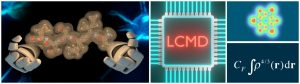
\includegraphics[scale=0.75]{lcmd-logo.jpg}
\end{minipage}
\vspace{0.5cm}
\hrule 
\vspace{0.5cm}
\begin{center}
\LARGE \textbf{\textcolor{red}{M}olecular \textcolor{red}{D}ynamics meets \textcolor{red}{N}eural \textcolor{red}{N}etworks}: \\
\LARGE \textbf{TUTORIAL}
\vspace{0.5cm}
\\ % The assignment title
\end{center}
\hrule 
\vspace{2cm}
\begin{center}
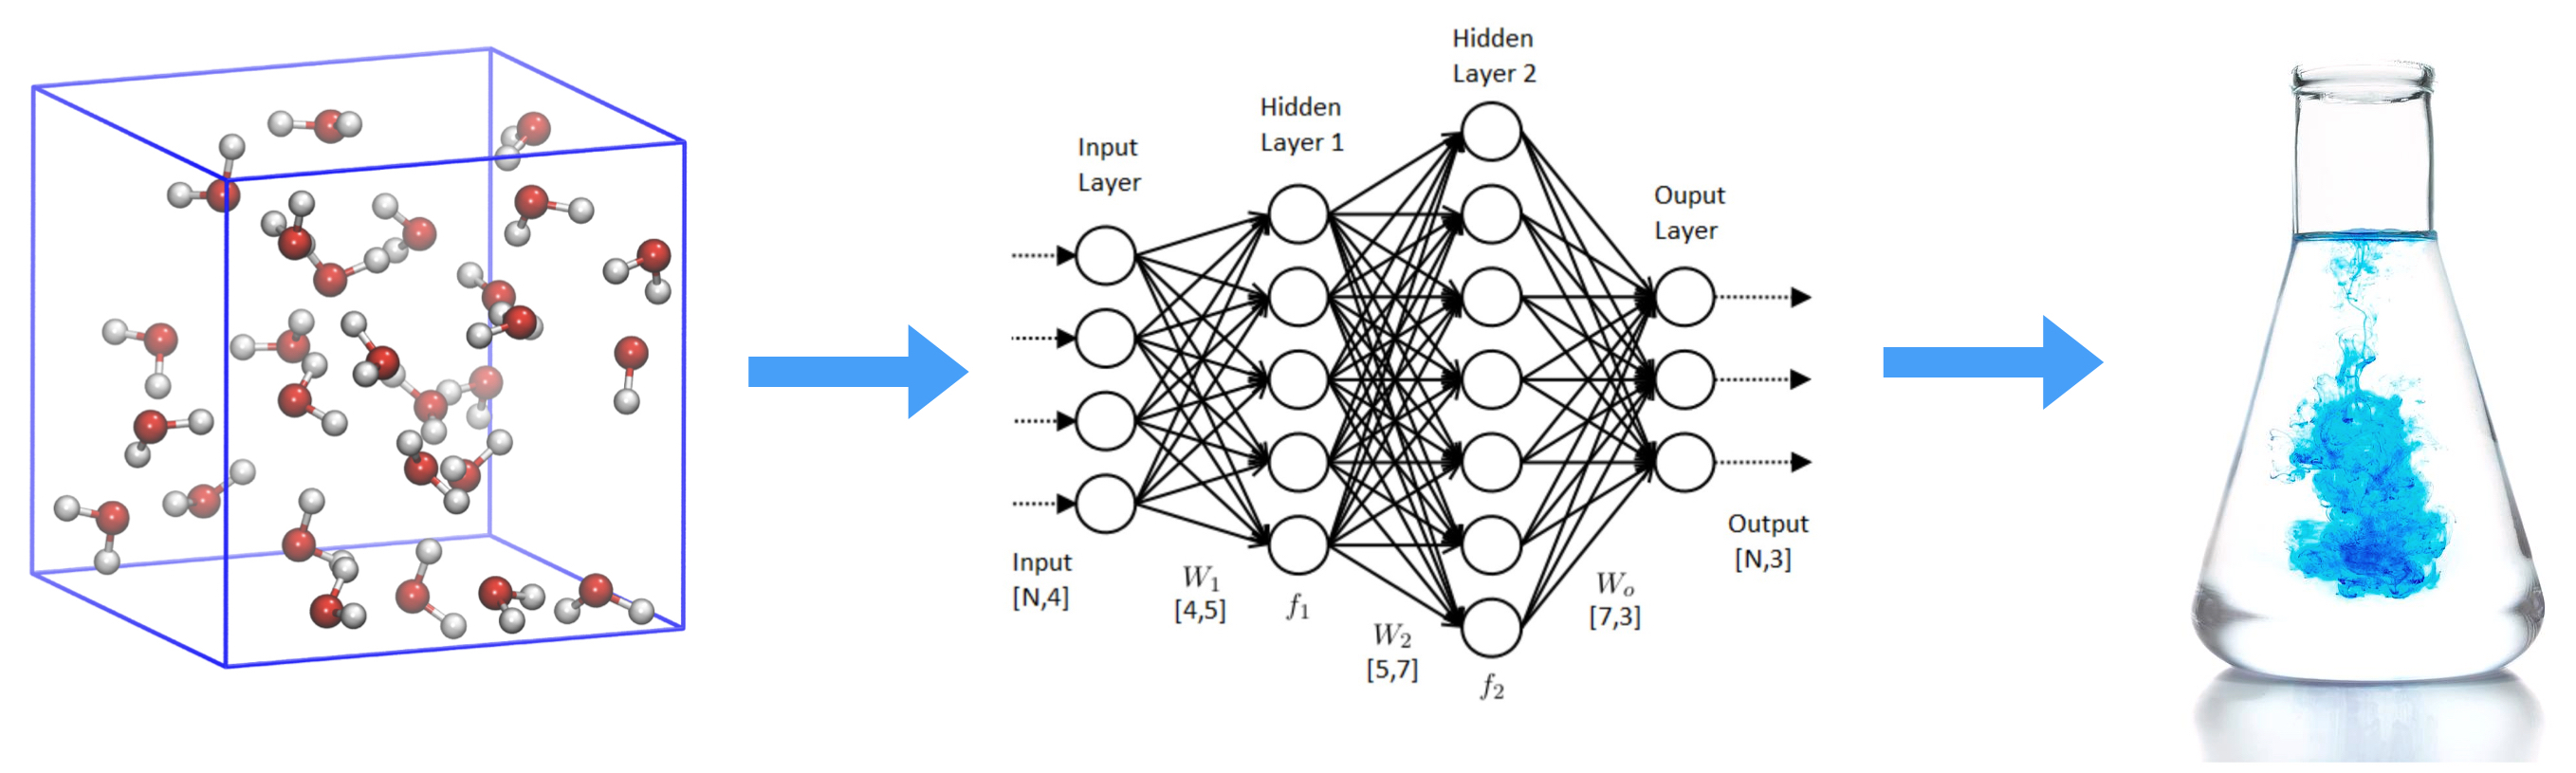
\includegraphics[scale=0.17]{Picture.jpeg}
\end{center}
\vspace{1cm}
\begin{center}
    Veronika JURÁSKOVÁ \\
    Frédéric CELERSE \\
    Rubén LAPLAZA \\
    Clémence CORMINBOEUF
\end{center}
%\vspace{2cm}
%\begin{mybox1}{}
%\Warning Please visit the website: \url{https://toto-is-coming-soon} to obtain last updates of this tutorial and information about other new tutorials.
%\end{mybox1}
 
% FIN PAGE DE PRESENTATION

% TABLE DES MATIERES
\newpage
\tableofcontents

% DEBUT DU TUTORIEL
\newpage
% SECTION INTRODUCTION
\pagestyle{fancy}
\renewcommand\headrulewidth{1pt}
\fancyhead[R]{MD combining NN: tutorial}
\renewcommand\footrulewidth{1pt}
\fancyfoot[C]{\thepage}
\fancyfoot[R]{\today}
\section{Introduction}
\fancyhead[L]{1. Introduction}
The aim of this tutorial is to provide a guidance for a building of the neural network-based potentials (NNPs) and their application in molecular dynamics (MD). As the traditional \textit{ab initio} MD is too computationally demanding for the description of chemical reactions and processes in large systems, the MD with NNPs benefits from much lower cost of the simulation while the accuracy it the AIMD is conserved.  %As chemical studies often involve reactions between two or more species, including such a feature in conventional  Born--Oppenheimer MD is commonly used in this context, however the numerical evaluation of energies and forces at the DFT level is extremely computationally demanding especially when applied to systems containing large number of atoms, \textit{e.g.} in the condensed phase. MD using a classical force field has been proposed as a solution to overcome this issue, but the form of the potential terms (\textit{i.e.}, harmonic) prevents bond breaking/forming in these simulations, limiting such approaches only to conformational sampling. \\ 
%In this tutorial, we describe how to enhance the speed of reactive systems simulation by exploiting the Neural Network-based potentials. 
In this regard, NNPs has been already used in the reactive simulations in gas phase and aqueous solutions (\textit{e.g.}, in the description of proton transfer and urea hydrolysis). %NNPs are trained to reproduce the energies (and possibly forces) of the accurate ab initio me. The main advantage of the NN is the low computational cost compare to pure Born--Oppenheimer DFT simulation. The NN based potentials are however still slower than a force field MD.

Part 1 of this tutorial is dedicated to the generation of the Behler-Parrinello NNPs, which represent the most complicated task of this tutorial as the preparation of a large and robust data set is time consuming and the accuracy of the training needs to be carefully monitored.

  %  \item It is time consuming to prepare sufficiently large and robust dataset; 
  %  \item Training properties (direct, $\Delta$, ...) play a crucial role in the prediction accuracy of the our MD/ML, so the training part has to be checked very carefully.

Part 2 demonstrates how to use the NNPs using the i--Pi interface to LAMMPS and other codes. Finally, Part 3 introduces the Baselined NNPs and showcase its advantages compared to standard NNPs trained directly on DFT data. %\textbf{It is important to note that even if final results do not provide chemical stability, the main importance of this tutorial is to provide you most important tools to understand how to deal with ML and MD. }
%\vspace{3cm}
%\begin{mybox1}{}
%\Warning All the data you need to follow this tutorial are freely available on the lcmdlc2 %local cluster at this adress: \textit{/home/celerse/Tutorial-fred-NNMD}
%\end{mybox1}
\newpage
%

\fancyhead[L]{2. Neural Networks-based potentials: Crash course}
\section{Neural Networks-based potentials: Crash course}
%
\subsection{Feedforward Neural Networks}
\begin{figure}[!h]
    \centering
    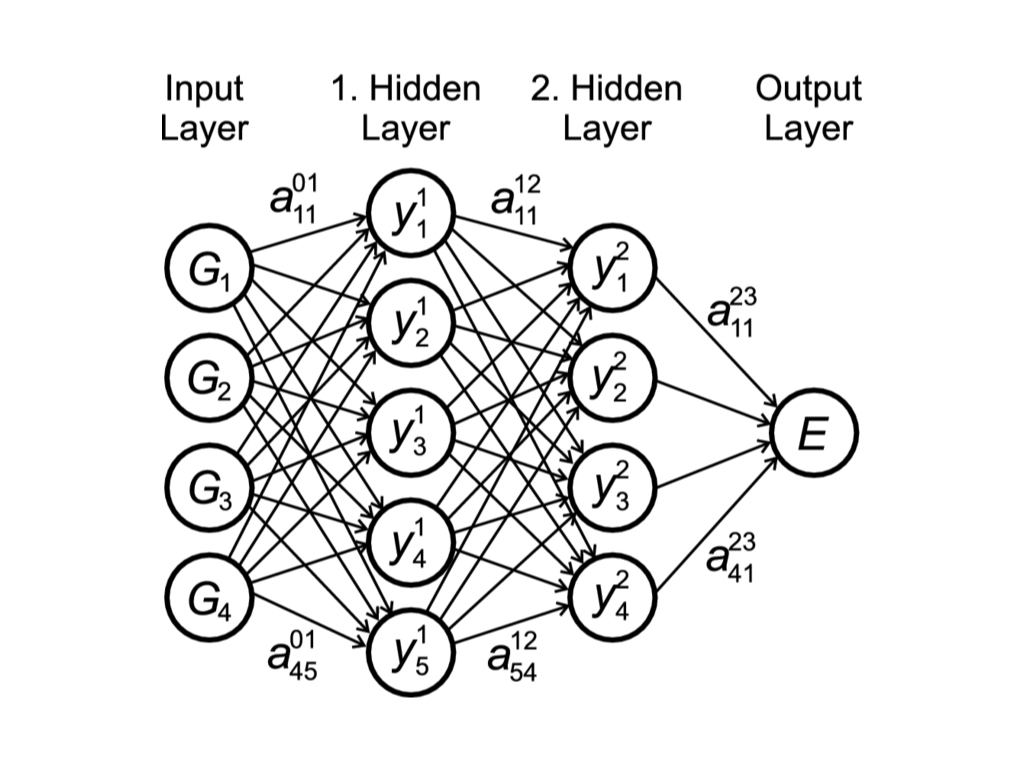
\includegraphics[scale=0.4]{NNP_scheme.jpeg}
    \caption{Schematic representation of a small feedforward NN. Nodes are interconnected in order to establish a functional relation between a set of coordinates $G$ (input layer) and the potential energy of the structure E (output layer). Notation of this NN is 4--5--4--1. }
    \label{NNP_scheme}
\end{figure}
\textbf{Neural Networks are statistical learning models which are able to reproduce complex non-linear mathematical functions, \textit{e.g.} the potential energy surface of molecular systems.} Using the so-called \textbf{data set}, the aim is to train the Neural Network Potentials (NNPs), which are used to propagate atom dynamics by estimating the shape of the potential energy surface. The forces are computed analytically as a negative gradient of the potential energy. As depicted in Fig. \ref{NNP_scheme}, the feedforward NN is made from number of nodes organized in several interconnected layers. The potential energy \textit{E} corresponds to the node in output layer and the atomic coordinates of a frame are provided in the input layer as a set of vector of input coordinates $G=\{G_i\}$. The input and output layers are connected via several so-called hidden layers with no physical meaning. The number of layers and the nodes defines the flexibility of the final NN. The example shows the NN with two layers containing five and four nodes, respectively. The short notation of such a NN is written as 4--5--4--1. The explanation of the notation is the following:
\begin{itemize}
    \item 4: Four nodes represent the input layer ($G_1$, $G_2$, $G_3$ and $G_4$);
    \item 5: Fives nodes in the first hidden layer;
    \item 4: Four nodes in the second hidden layer;
    \item 1: One node (the potential energy) in the output layer.
\end{itemize}
Each node is connected to all the nodes of the next layer with a specific weight \textbf{$a_{ij}^{kl}$}, where $i$ is the index of node of layer $k$, which is connected to the node with index $j$ of layer $l$. For instance, the $a_{45}^{01}$ connects the nodes $G_4$ ($k = 0$, $i=4$) and $y_5^1$ ($l=1$,  $j=5$). All the connections between nodes follow the same nomenclature. Not represented in our scheme, all the nodes in hidden and output layers are connected to so-called bias node, which scales their values by a bias weight b$_i^j$, where $j$ is the layer of the target node and $i$ the node index. 

The value y$_i^j$ of any node is computed as:
\begin{equation}
    y_i^{j} = f_i^j(b_i^j + \sum_{k=1}^{N_{j-1}} a_{k,i}^{j-1,j} y_k^{j-1})
\end{equation}
The equation is a linear combination of the values of all nodes in the previous layer scaled by the bias weight. The term f$_i^j$ represents the \textbf{activation function} of the NN. The activation function ensures the ability to fit complex non-linear functions. The examples of activation functions are:
\begin{itemize}
    \item hyperbolic tangent,
    \item sigmoid function,
    \item Gaussian function,
    \item Softplus
    \item trigonometric functions
    \item exponential function.
\end{itemize}
According to Figure~\ref{NNP_scheme}, the complete functional form for the energy is given by:
\begin{equation}
    E = f_1^3(b_1^3 + \sum_{k=1}^4 a_{k1}^{23} f_k^2 (b_k^2 + \sum_{j=1}^5 a{jk}^{12} f_j^1 (b_j^1 + \sum_{i=1}^4 a_{ij}^{01} G_i)))
\end{equation}

%The NNP constructed this way does not contain any information about the physics of the system. It simply links provided accurate electronic energy with the corresponding coordinates. The weight parameters in the NN are initially chosen as random numbers and are interativelly optimized to provide best estimation of the enrgy from given structure. However, the NN typically requi the longer the optimization process will be, but results will also be more precise. It is therefore important to find a good compromise between accuracy and dataset size This compromise has also to be reached regarding the number of nodes and layers, as increasing the number of nodes and layers also makes the optimisation slower but improve the accuracy.
%
\subsection{High--dimensional NNP}
\begin{figure}[!htp]
    \centering
    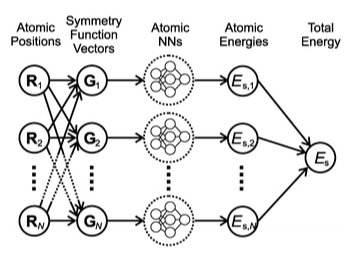
\includegraphics[scale=0.7]{High-dimensional-NNP_scheme.jpeg}
    \caption{High dimensional NN scheme: Atomic positions are represented by a vector of symmetry functions $G_i$. }
    \label{High-dimensional-NNP_scheme}
\end{figure}
Feedforward neural network discussed in previous section suffer from several drawbacks which prevented their application in the simulation of complex chemical systems. The limitations are for instance:
\begin{enumerate}
    \item absence of symmetry between equivalent terms (for instance, the OH bonds of a water molecule)
    \item system size dependency: no atoms could be deleted or added as it causes problems in the connecting weights).
\end{enumerate}
In 2007, Behler and Parrinello proposed a solution to this problem by expressing the total energy $E_s$ as a sum of the atomic energy contributions E$_i$.\cite{Behler2007}
\begin{equation}
    E_s = \sum_{i=1}^{N_{atom}} E_i
\end{equation}
Starting from the Cartesian coordinates $R$, every atom is represented by a set of atom-centered symmetry functions $G_i$, which describe the chemical environment of the atom within given cutoff. Each atom is then assigned a feedforward NN yielding the atomic contribution to the total energy. The weight of the NN are identical for atoms of the same element to ensure that the trained NNPs do not depend on the number and order of the atoms.
%
\subsection{Atom-centered symmetry functions}

Together with the NN topology, the seminal work of Behler and Parrinello introduced also new type of the symmetry functions to characterize the local environment of each atom. The so-called Atom-centered symmetry functions (ACSFs)\cite{behl11jcp} are constructed from the positions of the atoms and their closest neighbours. This representation guarantees that the atoms with the same environment yields the same atomic energy contribution which is also translationally and rotationally invariant. 

The typically used ACSFs are two-body radial and three-body angular functions in a form:

\begin{equation}
    G_i^2  = \sum_i e^{-\eta (R_{ij}-R_s)^2} \cdot f_c(R_{ij}) \label{eq:radial}
\end{equation}
\begin{equation}
    G_i^3  = 2^{(1-\xi)} \sum_{j,k \neq i}^{\mathrm{all}}(1 + \lambda \mathrm{cos}\;\theta_{ijk})^{\zeta} \cdot e^{-\eta (R_{ij}^2 + R_{ik}^2 + R_{jk}^2)} \cdot f_c(R_{ij}) \cdot f_c(R_{ik}) \cdot f_c(R_{jk}),
    \label{eq:angular}
\end{equation}

where $f_c$ is a cutoff function ensuring the smooth decay of the symmetry function to zero.   

In this tutorial, we use the original Behler-Parrinello ACSFs. However, during the last years many modifications to the original ACSFs were proposed as well as new types of functional forms to describe the atomic environments. Various types of structural representations are summarized for example in Ref. \citenum{Musil2021}.

%Symmetry function is a tool aiming at describing atomic configurations as a suitable set of coordinates. Indeed, a symmetry function needs to be suitable for the high--dimensional NNP problem, in other words, overcoming the invariance issue as well as to be independant of the number of atoms (in the cutoff spheres). Constructing such symmetry functions have been long time a major challenge in the advent of NNPs. As many type of symmetry functions exists, our choice in this tutorial is focused on the Behler--Parinello symmetry functions (ASFs), whihc are characterized by:

%Atom-centered symmetry functions (ACSFs) 
%
%\begin{itemize}
%    \item rotational and translational invariance
%    \item invariance with respect to the permutation of atoms of the same element
%    \item unique description of the atomic positions
%\end{itemize}
%
\subsection{Constructing and training NN}
The general protocol to construct NNP for a specific system is as follows:
\begin{enumerate}
    \item Define an initial set of structures and compute the reference energies and forces. The electronic structure method used as a reference should be accurate enough to describe the studied problem, but also not too computationally demanding as many single point computations are needed.
    \item Train first versions of NNP using the fraction of the data set. The remaining part of the set is used as a test set. Ideally, several different NNP with slightly different training sets should be trained to identify problems in the training set.
    \item Perform preliminary simulations using the NNPs to validate the stability of the NNP and find underrepresented areas of the PES, \textit{e.g.} structures triggering extrapolation warnings or unphysical geometries.
    \item Isolate the problematic structure, compute reference data and add them to the training set and re-train the NNP.
    \item Repeat the validation and re-training of the NNP until no instabilities are found and NNP are ready to be used.
\end{enumerate}

For detailed general tutorial review on Behler-Parrinello NN, see Ref. \citenum{Behler2015tutorial}. 

%
%\subsection{References}
\bibliographystyle{achemso}
\bibliography{bib}
%Complementary to the small explanation of the context of this tutorial, we strongly suggest to the reader a small list of articles which explain well the concept of NNP in more details:
%\begin{itemize}
%    \item Behler, J., Parrinello, M. (\textbf{2007}). Generalized neural-network representation of high-dimensional %potential-energy surfaces. \textit{Physical review letters}, 98(14), 146401.
%    \item Behler, J. (\textbf{2011}). Atom-centered symmetry functions for constructing high-dimensional neural network %potentials. \textit{The Journal of chemical physics}, 134(7), 074106.
%    \item Behler, J. (\textbf{2015}). Constructing high‐dimensional neural network potentials: A tutorial review. \textit{International Journal of Quantum Chemistry}, 115(16), 1032-1050.
%    \item Behler, J. (\textbf{2021}). Four generations of high-dimensional neural network potentials. \textit{Chemical Reviews}.
%\end{itemize}
%

\newpage
%

\fancyhead[L]{3. Requirements}
\section{Requirements}
This tutorial presents a workflow which requires extensive number of different software packages, scripts and libraries. The versions of the codes used here are listed below.

\subsection{Software}
All the codes are available at GitHub (see the last section of tutorial):
\begin{itemize}
    \item n2p2 (version 1.0.0)
    \item LAMMPS (version 2)
    \item i--PI (version 2.0)
    \item Tinker (version 8.8)
    \item cp2k (version 6.1)
\end{itemize}
%
\subsection{Dependencies}
\begin{itemize}
    \item python (version 2.7 and 3.6)
    \item libraries intel, intel-mpi, intel-mkl, gsl, eigen, gc,c mvapich2, openblas, n2p2/lib
\end{itemize}
%
%\subsection{Compilers}
%\begin{itemize}
%    \item gfortran (fortran compiler)
%    \item bash/shell (bash/shell compiler)
%    \item tclsh (tcl compiler)
%\end{itemize}
%
%
%
\newpage
%
\fancyhead[L]{4. Building NNPs}
\section{Part 1: How to generate neural network potentials}
\subsection*{Instructions}
%Generating a Machine Learning Potentials (M is not of an easy task. Indeed, our approach depicts quite transferability between systems and prepared MLP as one MLP is dedicated to one system. Future works will be provided in this direction. For one specific system, generating a MLP following our procedure results in:

Currently, there is no universal NNP which is applicable to model all classes of systems. Despite ongoing effort in the training of general neural network-based force-fields, many system require building of the NNPs from scratch. In the following section, we provide general instructions how to train NNP using Behler-Parrinello NN. The required steps include: 

\begin{enumerate}
    \item Generating initial data;
    \item Careful selection of a database of structures in order to provide the best representation of the conformational space while keeping the number of structures relatively low;
    \item Computation of reference forces and energies for all the selected structures;
    \item Training of the NN.
\end{enumerate}
%
\subsection{Step 0: The system}
\begin{figure} [!htp]
    \centering
    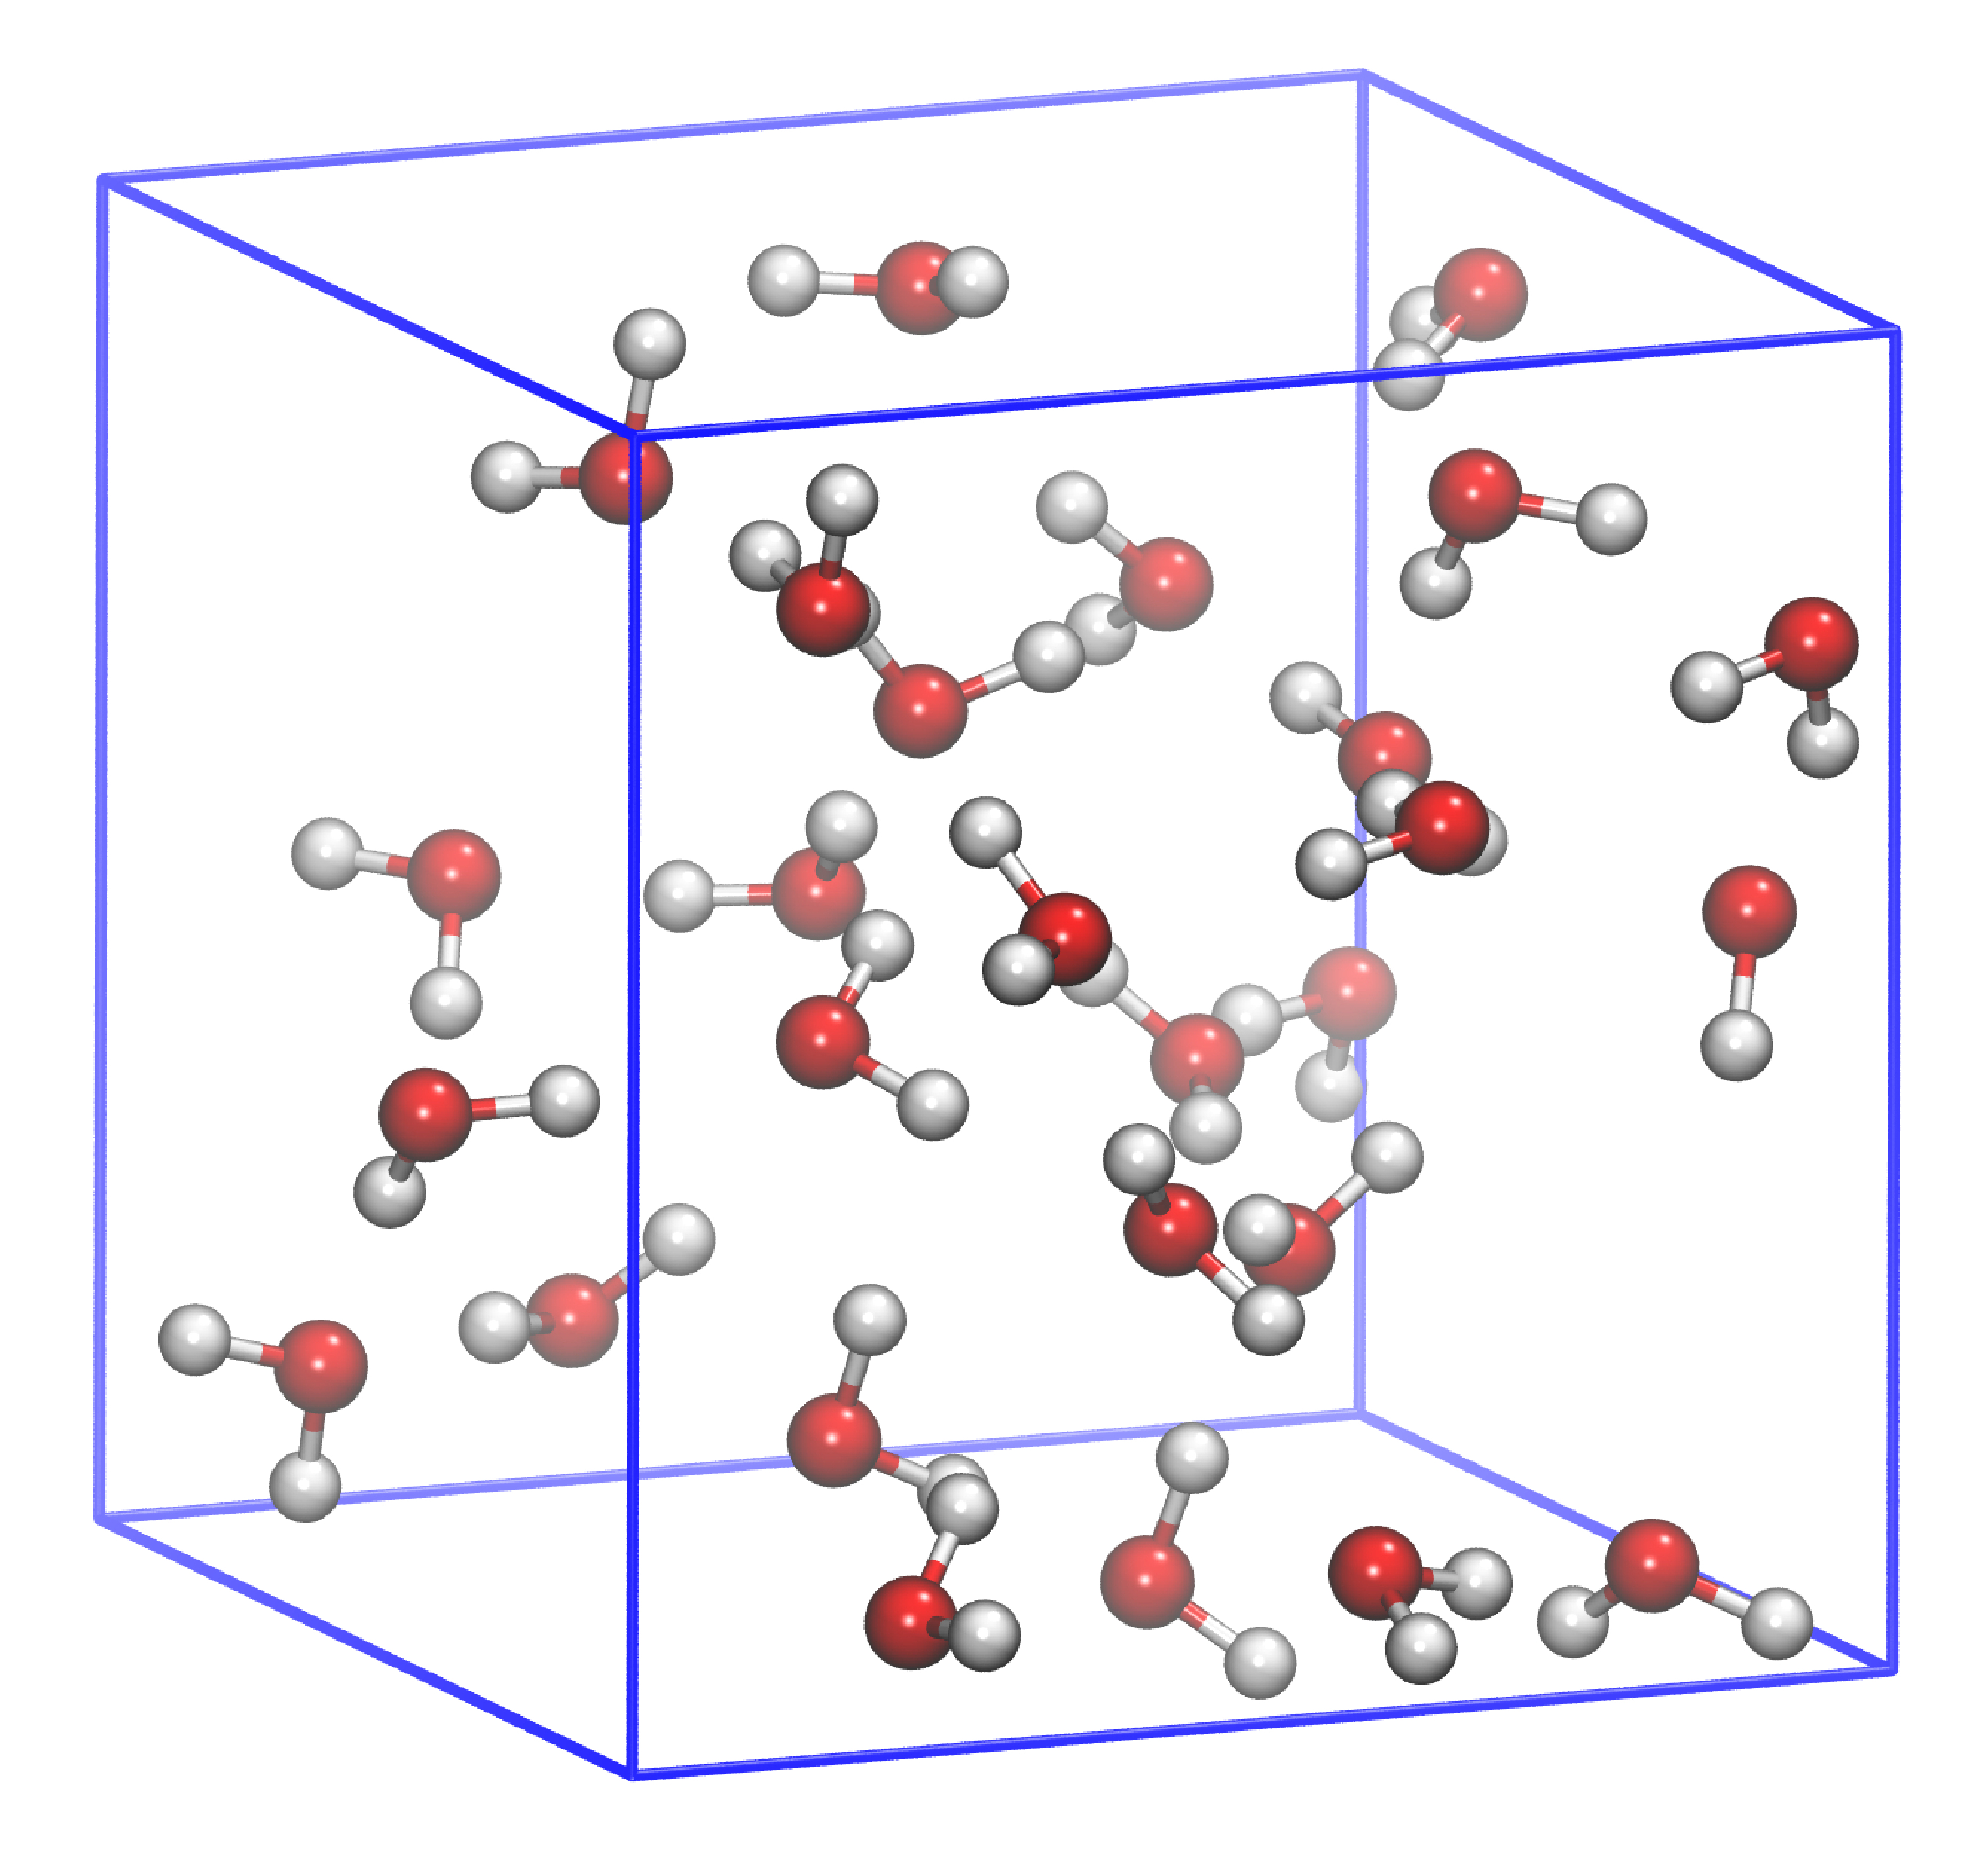
\includegraphics[scale=0.05]{watertiny.jpeg}
    \caption{System containing 27 molecules in a cubic box with edge of 9.32 \AA.}
    \label{Rep_sys}
\end{figure}
%As we need to choose a practical system (which is not too big) in order to facilitate the understanding of this tutorial, our choice was focused on a tiny water box of 81 atoms (eg 27 water molecules, see Figure~\ref{Rep_sys}). A cubic waterbox of dimension 9.32 \AA~ has been considered. The aim is thus to be able to reproduce as accurately as possible the energetics and forces occurring in the system in different conformations during a MD/ML.
 
%

As a relatively simple test case, we train the NNPs for a small water box containing 27 water molecules with the cell size of 9.32 \AA. This systems contain only two elements, \textit{i.e.} H and O, which significantly simplifies the training.

\subsection{Step 1: Generating the data}
\begin{mybox2}{{Files needed}}
\begin{minipage}[c]{0.5\linewidth}

\includegraphics[scale=0.2]{tinker.png}
\end{minipage}
\begin{minipage}[c]{0.5\linewidth}
\begin{itemize}
    \item system.xyz
    \item system.key
    \item system.dyn
    \item water03.prm
    \item \textit{dynamic} module
\end{itemize}
\end{minipage}
\end{mybox2}
The first step in the tutorial is the preparation of the training set. The training set can be build from systems with different size and different compositions. To keep things simple, we will train the NNPs using only one size of the water box defined above. To generate extensive set of the structures, it is beneficial to use molecular dynamics starting either from equilibrated structure or from experimental data (\textit{e.g.}, X-ray). Random displacement of the atoms could be also applied.
%\begin{enumerate}
%    \item classical Molecular Dynamics (cMD) using non--polarizable force fields (n--PFF);
%    \item cMD using polarizable force fields;
%    \item Hybrid DFT MD (DFTB+, xtB, orca, ...)
%    \item Born--Openheimer MD (Quantum espresso, cp2k, ...)
%\end{enumerate}

%As the aim is to generate maximum of data at this point, MD should be fast enough to roughly sample the phase space. However, the dataset should be made off realistic structures, thus we decided to choose as a good compromise between accuracy and speed the cMD combining with the use of polarizable force field. \\

As the first training set should be large enough but also contain meaningful geometries, the potential for the exploratory dynamics should represent good cost/accuracy ratio. For example, classical force-fields might not be the best choice, as they can sample structures which are too different from the ones obtained at the reference level. The reasonable compromise are therefore semiempirical methods or polarizable force-fields.

In this tutorial, we generate the system using AMOEBA polarizable force-field as available in Tinker. The files required for the simulation are *.xyz,  *.key and *.prm. For more information on the preparation of the files for Tinker, see tutorials listed in section \ref{sec:tutorials}.

Here, we just briefly comment on the content of the files:

\begin{itemize}
    \item The .xyz file contains the Cartesian coordinates of the initial water box in the Tinker xyz format (Caution! Tinker xyz differs significantly from standard xyz or extended xyz formats.)  
    \item The .key file has the role of an input file. It contains the settings to run the dynamics.
    \item The .dyn serves as a restart file. It contains positions, velocities and accelerations of the last frame of the dynamics.
    \item The .prm file corresponds to the AMOEBA parameters. It contains all the terms to compute the potential energy of a specific structure.
\end{itemize}

%The simplest as the fastest way to perform a cMD is to launch only 1 in a specific direction. Therefore, on your cluster you first need to place all these files (system.xyz, system.key and water03.prm) in a same directory. Once this is done, you could easily launch your dynamics using the following command line (if the \textcolor{green}{dynamic} module is in your bin directory):
MD using Tinker can be launched by a following command:
\begin{center}
\mybox{\textit{dynamic system 1000000 2.0 1 2 300 $>$ system.out}}
\end{center}
This command means that the simulation will run using the \textit{dynamic} module for 1000000 steps with a time step of 2.0 fs (\textit{i.e.}, the total length of the simulation is 2 ns). The next term specifies the frequency (in ps) of saving the trajectory to the .arc file, here we save it every 1 ps. The final system.arc file will thus contain 2000 frames. The following term specifies the mode of the dynamics, 2 corresponds to NVT canonical ensemble. The last term corresponds to the temperature of the simulation, here it is set to 300 K. 

\begin{mybox1}{Enhanced sampling}
\Warning As our system is quite simple, the standard molecular dynamics is sufficient to provide extensive sampling. In more complex cases, however, the simulations starting from different initial structures or using enhanced sampling techniques might be needed to ensure that all the relevant structures are present. Suitable simulations techniques include for instance:
\begin{enumerate}
    \item Replica exchange molecular dynamics
    \item Sampling techniques using bias, such as metadynamics, steered molecular dynamics, umbrella sampling, ...
    \item Transition path sampling
\end{enumerate}
\end{mybox1}
\begin{mybox1}{Extending the database with more distorted structures}
\Warning The NNPs have in general very limiting extrapolation capacity. As their are trained only on the information included in the training set, it is beneficial to consider more distorted structures covering the repulsive and dissociative parts of the PES. Distorted structures can be generated by simulations using for example: 
\begin{enumerate}
    \item High temperature
    \item High pressure
    \item Path integral molecular dynamics
    \item Specific constraints and restraints
    \item Random displacement
\end{enumerate}

\end{mybox1}
\begin{mybox3}{Output Files}
\begin{itemize}
    \item system.out
    \item \textbf{system.arc} (file containing the structures)
    \item system.dyn
\end{itemize}
\end{mybox3}
%
\subsection{Step 2: Database selection}
\subsubsection{Preparing files for n2p2}
\begin{mybox2}{{Input Files, Executables and Scripts}}
\begin{minipage}[c]{0.5\linewidth}

\includegraphics[scale=0.1]{Python-fortran.jpeg}
\end{minipage}
\begin{minipage}[c]{0.5\linewidth}
\begin{itemize}
    \item system.arc
    \item \textcolor{red}{from\_txyz\_to\_n2p2.f90}
    \item \textcolor{red}{symmtery\_functions.py}
\end{itemize}
\end{minipage}
\end{mybox2}
Once the initial data are generated, we need to select small set of structures which will be used to prepare a set of symmetry functions.  
Let's assume that all generated structures are present in system.arc file. 
%When more than 1 trajectory is performed, all the system.arc should be concatenated. If for instance you ran 5 independent MD, you should rename each .arc files as system1.arc / system2.arc / system3.arc / system4.arc / system5.arc and concatenate them in one single .arc file as:
%\begin{center}
%\mybox{\textit{cat system1.arc system2.arc system3.arc system4.arc system5.arc $>$ SYSTEM-TOT.arc}}
%\end{center}
%In this case, while we only have on single .arc file we will continue with the system.arc file. \\
%The first thing to do is to convert each frame of the system.arc file in the right format for the n2p2 software. This file, named \textbf{input.data}, has to contain all the considered structures. You could prepare this file following this procedure:

Structures in this file can be converted to input files for n2p2 as follows:

\begin{enumerate}
    \item compile the fortran code \textcolor{red}{from\_txyz\_to\_n2p2.f90}:
    \textit{gfortran from\_txyz\_to\_gen.f90 -o from\_txyz\_to\_gen} 
    \item place the system.arc file in the same directory of the \textcolor{green}{from\_txyz\_to\_gen} executable and launch it as \textit{./from\_txyz\_to\_gen}
\end{enumerate}
The script generates input.data file for the n2p2 containing all the structures. The definition of every structure starts with a short header:

 begin \\
 comment \\
 lattice 17.612 0.0 0.0 \\
 lattice 0.0 17.612 0.0 \\
 lattice 0.0 0.0 17.612 \\

"begin" and "comment" are present at the beginning of every new structure. "lattice" defines the dimension of the box. The units of the box and Cartesian coordinates are converted to Bohr.
Each atom of the structure is defined as: \\ \\
 atom \hspace{0.5cm}  -4.367  \hspace{0.5cm}      5.267    \hspace{0.5cm}    4.603  \hspace{0.5cm}    O \hspace{0.5cm} 0 0 \hspace{0.5cm} 0.0 0.0 0.0 \\ \\
The keyword "atom" specify that the line corresponds to one atom, -4.367, 5.267, 4.603 are the xyz coordinates of the atom, O is the element label, the following two columns 0 0 are not used  and, finally, the last three columns 0.0 0.0 0.0 are the xyz force components acting on the atom. At this example, forces are set to 0.0 since they are not used.

The file ends with: 

 energy 0.000 \\
 charge 0.0 \\
 end \\

where "energy" is the reference total energy of the system, "charge" is the total charge of the system, and "end" closes the definition of the structure. 

\begin{mybox1}{Units in n2p2}
\Warning As indicated on the n2p2 website, the units correspond to the physical units defined in the input files. As we are combining several different codes which might have different unit specifications, keep track on the units and stay consistent within the workflow.

In the inputs for n2p2, we use units as:
\begin{enumerate}
    \item lattice: \textbf{Bohr}
    \item x/y/z positions: \textbf{Bohr}
    \item x/y/z forces: \textbf{Hartree Bohr$^{-1}$}
    \item energy: \textbf{Hartree}
\end{enumerate}

\textcolor{red}{The conversion from Angström to Bohr is done by a multiplication by a factor \textbf{1.88973}}
\end{mybox1}

The next file to prepare is the \textbf{input.nn} file, which corresponds to the parameters given to parametrize our Neural Network. It is made off three parts:
\begin{enumerate}
    \item GENERAL NNP SETTINGS
    \item ADDITIONAL SETTINGS FOR TRAINING
    \item SYMFUNCTIONS
\end{enumerate}
GENERAL NNP SETTINGS correspond to the general settings we give to the Neural Network, as the name and number of elements, the number of layers and nodes, activation function for each hidden layer and output layer, etc. \\
ADDITIONAL SETTINGS FOR TRAINING are complementary information enabling to parametrize the neural network. \\
As points 1 and 2 are often already fixed by using some conventional parameters used in previous work, the last thing to generate is the symmetry functions (symfunctions). In our case we employ Behler--Parrinello atomic symmetry functions (ASFs) as an input to a feed--forward neural network. We have to generate them for atoms O and H, we thus employ the python script \textcolor{red}{symfun\_gen.py} by typing in the terminal:
\begin{center}
\mybox{\textit{python symfun\_gen.py $>$ asfs.txt}}
\end{center}
Without any arguments, \textcolor{red}{symfun\_gen.py} generates the data by default: ASFs for only H atom, with a cutoff of 12.0 Bohr and a delta of 0.05. If you want more (as it surely the case), please add in the sumbission line the following different options:
\begin{itemize}
    \item -e: the name of elements we want the symmetry functions (default: H) (example in this case: -e H O)
    \item -c: the cutoff for the symmetry functions (default: 12.0) (example in this case: -c 14.0)
    \item -d: the ratio between the minimum sigma of the gaussian and the cutoff. It determines the accuracy with which you sample the space. (default: 0.05) (example in this case: -d 0.2)
\end{itemize}
According to these parameters and the system we want to use, the submission line for \textcolor{red}{symfun\_gen.py} becomes:
\begin{center}
overleaf color boxex grey \mybox{\textit{python symfun\_gen.py -e H O -c 14.0 -d 0.2 $>$ asfs.txt}}
\end{center}
ASFs are thus generated and stocked in the asfs.txt file, which could then be concatenated to the input.nn as:
\begin{center}
\mybox{\textit{cat input.nn asfs.txt $>$ toto ; mv toto input.nn}}
\end{center}
We thus have two initial files:
\begin{itemize}
    \item \textbf{input.data}
    \item \textbf{input.nn}
\end{itemize}
which are the base to launch n2p2 computations.
\\
\begin{mybox3}{Output Files}
\begin{itemize}
    \item \textbf{input.data}
    \item \textbf{input.nn} 
\end{itemize}
\end{mybox3}
%
\subsubsection{Launching first computations with n2p2}
\begin{mybox2}{{Input Files, Executables and Scripts}}
\begin{minipage}[c]{0.5\linewidth}

\includegraphics[scale=0.1]{n2p2.png}
\end{minipage}
\begin{minipage}[c]{0.5\linewidth}
\begin{itemize}
    \item input.data
    \item input.nn
    \item \textcolor{green}{nnp--scaling}
    \item \textcolor{red}{CurSel-integral.py}
    \item \textcolor{red}{curlib.py} / \textcolor{red}{iolib.py} / \textcolor{red}{sflib.py}
\end{itemize}
\end{minipage}
\end{mybox2}
The first step, once initial files .data and .nn are ready, is to launch the scaling of our neural network. To perform this task you could place in the same directory the .data and .nn files and type in your terminal:
\begin{center}
\mybox{\textit{mpirun -n 32 nnp-scaling 500 $>$ logfile}}
\end{center}
\begin{mybox4}{Libraries}
\begin{itemize}
    \item module load intel intel-mpi intel-mkl gsl eigen is adviced !
    \item module load n2p2 if available !
    \item specify your n2p2 libraries path as: \\ "export LD\_LIBRARY\_PATH=\$LD\_LIBRARY\_PATH:$<$path-to-your-n2p2-lib$>$"
\end{itemize}
\end{mybox4}
3 output files are thus generated:
\begin{enumerate}
    \item \textbf{logfile}: all instructions occuring in the nnp--scaling procedure are listed in this file. It is also very useful as it evaluates the memory for all structures. \textbf{A rule of thumb is that it should not exceed 100 GB.}
    \item \textbf{function.data}: all the functions for our system are listed in this file, which is very memory consuming. So do not try to open it manually.
    \item \textbf{scaling.data}: nnp--scaling procedure compute all symmetry functions for all atoms once and store statistics about them in this file, required after for training.
\end{enumerate}
Among all the ASFs generated, it is now essential to choose a reasonably as well as nonredundant set of ASFs which describe as accurately as possible our system. This task is often the most delicate and time--consuming aspects in the construction of a Behler--Parinnello style MLP. We thus decided to automatize this selection using CUR description and implemented in a home script named \textcolor{red}{CurSel-integral.py}. You could just place this script in the same direction as function.data and launch it as:
\begin{center}
\mybox{\textit{python CurSel-integral.py function.data logfile -n 64 --landmarks 1000 --prefix cursel $>$ out}}
\end{center}
As before, 3 output files are generated:
\begin{enumerate}
    \item \textbf{out}: the output file of the procedure.
    \item \textbf{cursel.def}: the chosen symmetry functions.
    \item \textbf{cursel.landmarks}: the frame's number selected.
\end{enumerate}
The \textbf{cursel.def} will be useful in the STEP 4 and \textbf{cursel.landmarks} in STEP 3. \\
\begin{mybox1}{Checking of the ASFs !}
\Warning Generated ASFs  should be checked by plotting them in an external software (gnuplot) in order to check if they well cover the space or not. A good balance between G2 and G3 has also to be respected !
\end{mybox1}
\begin{mybox1}{Stability of NNP !}
\Warning Although a good balance between G2 and G3 is needed, some other parameters are important to consider. One of them is the number of structures within the dataset. In our case, with only 1000 structures we can not wait for a stable NNP as the number of structures should not be sufficient enough. However, we kept this number to ensure a good ratio between understanding and short computational time for methodological understanding within this tutorial. However, this setup should not be used for production. If the user is then, after this tutorial, interested to use it for production, a setup used recently for production is provided at the end of this tutorial ! 
\end{mybox1}


\begin{mybox3}{Output Files}
\begin{itemize}
    \item logfile
    \item function.data
    \item scaling.data
    \item out
    \item \textbf{cursel.def}
    \item \textbf{cursel.landmarks}
\end{itemize}
\end{mybox3}
%
\subsection{Step 3: Hybrid DFT force--energy computations}
\subsubsection{Extracting structures of interest}
\begin{mybox2}{{Input Files, Executables and Scripts}}
\begin{minipage}[c]{0.5\linewidth}

\includegraphics[scale=0.1]{Python-fortran.jpeg}
\end{minipage}
\begin{minipage}[c]{0.5\linewidth}
\begin{itemize}
    \item cursel.landmarks
    \item input.data
    \item \textcolor{red}{selection.f90}
    \item \textcolor{red}{from\_data\_to\_xyz.f90}
    \item \textcolor{red}{from\_xyz\_to\_cp2k.f90}
\end{itemize}
\end{minipage}
\end{mybox2}
From the cursel.landmarks file generated in the previous step, we need to extract structures in order to perform single point reference computations. From the input.data file you could apply a home script \textcolor{red}{selection.f90} as:
\begin{center}
\mybox{\textit{gfortran selection.f90 -o selection ; ./selection}}
\end{center}
It will generate a newfile labeled as \textbf{new--input.data} and containing the 1000 selected structures from the CUR procedures. 

The next steps is now to extract each structures and to place them in an individual file for enabling cp2k computations. This procedure corresponds, once again, to post--processing and could be performed in a two step way following this procedure:
\begin{enumerate}
    \item \textit{gfortran from\_data\_to\_xyz.f90 -o from\_data\_to\_xyz ; ./from\_data\_to\_xyz}
    \item \textit{gfortran from\_xyz\_to\_cp2k.f90 -o from\_xyz\_to\_cp2k ; ./from\_xyz\_to\_cp2k}
\end{enumerate}
You obtain a series of 1000 files named \$i-cp2k.xyz, which corresponds to the 1000 initial structure files for cp2k computations.
\\
\begin{mybox3}{Output Files}
\begin{itemize}
    \item \textbf{\$i-cp2k.xyz}
\end{itemize}
\end{mybox3}
%
\subsubsection{CP2K computations}
\begin{mybox2}{{Input Files, Executables and Scripts}}
\begin{minipage}[c]{0.5\linewidth}

\includegraphics[scale=0.1]{CP2K_logo.png}
\end{minipage}
\begin{minipage}[c]{0.5\linewidth}
\begin{itemize}
    \item \$i-cp2k.xyz
    \item input.cp2k
    \item \textcolor{red}{prep-file.sh}
\end{itemize}
\end{minipage}
\end{mybox2}
We firstly need to prepare one directory for one calculation. This task could be automatized using the \textcolor{red}{prep-file.sh} bash file which automatically create you 1000 directories, one per frame. Each of them contain one .xyz file and .cp2k file. The input.cp2k file is where we place specific keywords to parametrize the cp2k computations. In our case, we are using the CP2K 6.1 version to perform reference energies and forces at the PBE--D3BJ level of theory. All elements are described with the TZV2P--MOLOPT basis set with cores represented by the dual--space Goedecker--Teter--Hutter pseudopotentials (GTH PBE). The plane--wave cutoff is set to 700 Ry with a relative cutoff of 70 Ry. All computations employ a Coulomb operator truncated at R=6 \AA~ and the auxilary de,sity matrix method with a cpFIT3 fiiting basis set. \\ \\
To launch a cp2k calculation, just type in the directory of your .xyz and .cp2k files the following command:
\begin{center}
\mybox{\textit{cp2k.popt -i input.cp2k -o output.cp2k}}
\end{center}
A series of files will be generated, but the most important in our case is the \textbf{output.cp2k} file. This task has to be performed for the 1000 structures, \textbf{each calculation is taken 3 minutes on 28 CPUs approximatively}. 
\\
\begin{mybox3}{Output Files}
\begin{itemize}
    \item \textbf{output.cp2k} 1000 times !
\end{itemize}
\end{mybox3}
%
\subsubsection{Extraction of forces and energies}
\begin{mybox2}{{Input Files, Executables and Scripts}}
\begin{minipage}[c]{0.5\linewidth}

\includegraphics[scale=0.1]{Python-fortran.jpeg}
\end{minipage}
\begin{minipage}[c]{0.5\linewidth}
\begin{itemize}
    \item output.cp2k 1000 times !
    \item \textcolor{red}{extraction.tcl}
    \item \textcolor{red}{trait.sh}
\end{itemize}
\end{minipage}
\end{mybox2}
From each output.cp2k generated in the previous step, we need now to extract the potential energy term and x/y/z component forces acting on each atoms of the structure. A classical tcl file named \textcolor{red}{extraction.tcl} has been designed to automatized this task. In the directory of your output.cp2k you could just launch:
\begin{center}
\mybox{\textit{tclsh extraction.tcl}}
\end{center}
It will generate an outputfile named \textbf{output-forces.dat}. The procedure can be easily automatized for the 1000 directories by using a classical bash file named \textcolor{red}{trait.sh} and launched in the directory of the 1000 directories (and one copy of the extraction.tcl file)  as:
\begin{center}
\mybox{\textit{sh trait.sh}}
\end{center}
It will generate a final output named \textbf{forces\_and\_energies.dat}, containing all the information of your 1000 structures. 
\\
\begin{mybox3}{Output Files}
\begin{itemize}
    \item \textbf{forces\_and\_energies.dat}
\end{itemize}
\end{mybox3}
%
\subsubsection{Updating the input.data file}
\begin{mybox2}{{Input Files, Executables and Scripts}}
\begin{minipage}[c]{0.5\linewidth}

\includegraphics[scale=0.1]{Python-fortran.jpeg}
\end{minipage}
\begin{minipage}[c]{0.5\linewidth}
\begin{itemize}
    \item input.data
    \item forces\_and\_energies.dat
    \item \textcolor{red}{update.f90}
\end{itemize}
\end{minipage}
\end{mybox2}
After obtaining forces and energies for each of our structures, we need to inject them within our initial input.data file. A home script named \textcolor{red}{update.f90} has been designed to perform this task and could be launched in the same directory as the input.data and forces\_and\_energies.dat files as:
\begin{center}
\mybox{\textit{gfortran update.f90 ; ./a.out}}
\end{center}
You now have to replace your old input.data by the \textbf{new-input.data} generated as the output of your script for the next step.
\\
\begin{mybox3}{Output Files}
\begin{itemize}
    \item \textbf{input.data} (renamed after being new-input.data)
\end{itemize}
\end{mybox3}
%
\subsection{Step 4: Neural Network Potential training}
\subsubsection{Regenerate new scaling.data file}
\begin{mybox2}{{Input Files, Executables and Scripts}}
\begin{minipage}[c]{0.5\linewidth}

\includegraphics[scale=0.1]{n2p2.png}
\end{minipage}
\begin{minipage}[c]{0.5\linewidth}
\begin{itemize}
    \item input.data
    \item input.nn
    \item \textcolor{green}{nnp--train}
\end{itemize}
\end{minipage}
\end{mybox2}
Before proceeding to the Neural Network training a new scaling.data has to be generated, with use of the new files created during the previous steps:
\begin{itemize}
    \item input.data, coming from the "Updating the input.data file";
    \item input.nn, coming from "Preparing files for n2p2"
\end{itemize}
You create a new directory encompassing these two files and applied the \textcolor{green}{nnp--scaling} procedure similarly to the point "Preparing files for n2p2" in order to generate the right scaling.data file. 
\\
\begin{mybox3}{Output Files}
\begin{itemize}
    \item \textbf{scaling.data}
\end{itemize}
\end{mybox3}
%
\subsubsection{Training our Neural Network}
\begin{mybox2}{{Input Files, Executables and Scripts}}
\begin{minipage}[c]{0.5\linewidth}

\includegraphics[scale=0.1]{n2p2.png}
\end{minipage}
\begin{minipage}[c]{0.5\linewidth}
\begin{itemize}
    \item input.data
    \item input.nn
    \item scaling.data
    \item \textcolor{green}{nnp--train}
\end{itemize}
\end{minipage}
\end{mybox2}
Once this step done, you create another directory encompassing this time:
\begin{itemize}
    \item input.data
    \item input.nn
    \item scaling.data
\end{itemize}
and you launch your training procedure as:
\begin{center}
\mybox{\textit{mpirun -n 32 nnp--train $>$ output.txt}}
\end{center}
\begin{mybox4}{Libraries}
\begin{itemize}
    \item module load intel intel-mpi intel-mkl gsl eigen is adviced !
    \item specify your n2p2 libraries path as: \\ "export LD\_LIBRARY\_PATH=\$LD\_LIBRARY\_PATH:$<$path-to-your-n2p2-lib$>$"
\end{itemize}
\end{mybox4}
Several files are created, but the most interesting are:
\begin{itemize}
    \item \textbf{output.txt}: it is the main output file of the calculation. Initial parameters for the training procedure is listed to avoid some troubles in the initial setting. Sum of the training computations each epoch are listed with for each one the calculation time. 
    \item \textbf{learning--curve.out}: this is the main file to easily plot the different learning curves using an external software.
    \item \textbf{weights}: for each atom a weight file is created. For instance as H is 1, for the epoch 120 you should obtain "weights.001.120.out". These files are a sum of all the weights used in the Neural Network connections (see the few reminder part on the NN). These files are crucial when the procedure should be restarted (see next subpart). 
\end{itemize}
Be focused now on the \textbf{learning--curve.out} file. It is presented in 5 columns:
\begin{enumerate}
    \item Column 1: the current epoch
    \item Column 2: RMSE of training energies per atom (physical units)
    \item Column 3: RMSE of test energies per atom (physical units)
    \item Column 4: RMSE of training forces (physical units)
    \item Column 5: RMSE of test forces (physical units)
\end{enumerate}
To ensure the stability of our NN, we have to check the RMSE values obtained in function of the epoch. This could be performed in two steps:
\begin{enumerate}
    \item Firstly, we check the quality of the energy prediction: a good compromise should be an error around 1 meV/atom. If it is higher, be careful and you need to check the stability of your NN when you will branch it to your MD.
    \item Secondly, we check the quality of the forces prediction: as forces are more complicated to be predicted compared to the energy, a good compromise between accuracy and prediction should be an error around 150 meV/atom. As for the energy, if its higher you need also to check the stability of your NN when it will be branched to your MD. 
\end{enumerate}
Results obtained in this file are in the cp2k units, so in our case it is in a.u (atomic units, you could easily check it in an output.cp2k you obtained previously). It is thus desirable to translate a.u in meV/atom. \\
Conversion: 1 a.u = 627.5 kcal/mol = 27.211 eV, so to pass from a.u to meV the factor to apply is 27211 for the energy. Concerning the forces, a factor 2 has to be added. As results are average taken on the atoms, the final result is in meV/Atom (so do not need to divide it by the number of atoms). Using an external software to plot the curves (python, gnuplot, xmgrace, excel, ...) you should be able to obtain these curves depicted on Figure. 
\begin{figure}
    \centering
    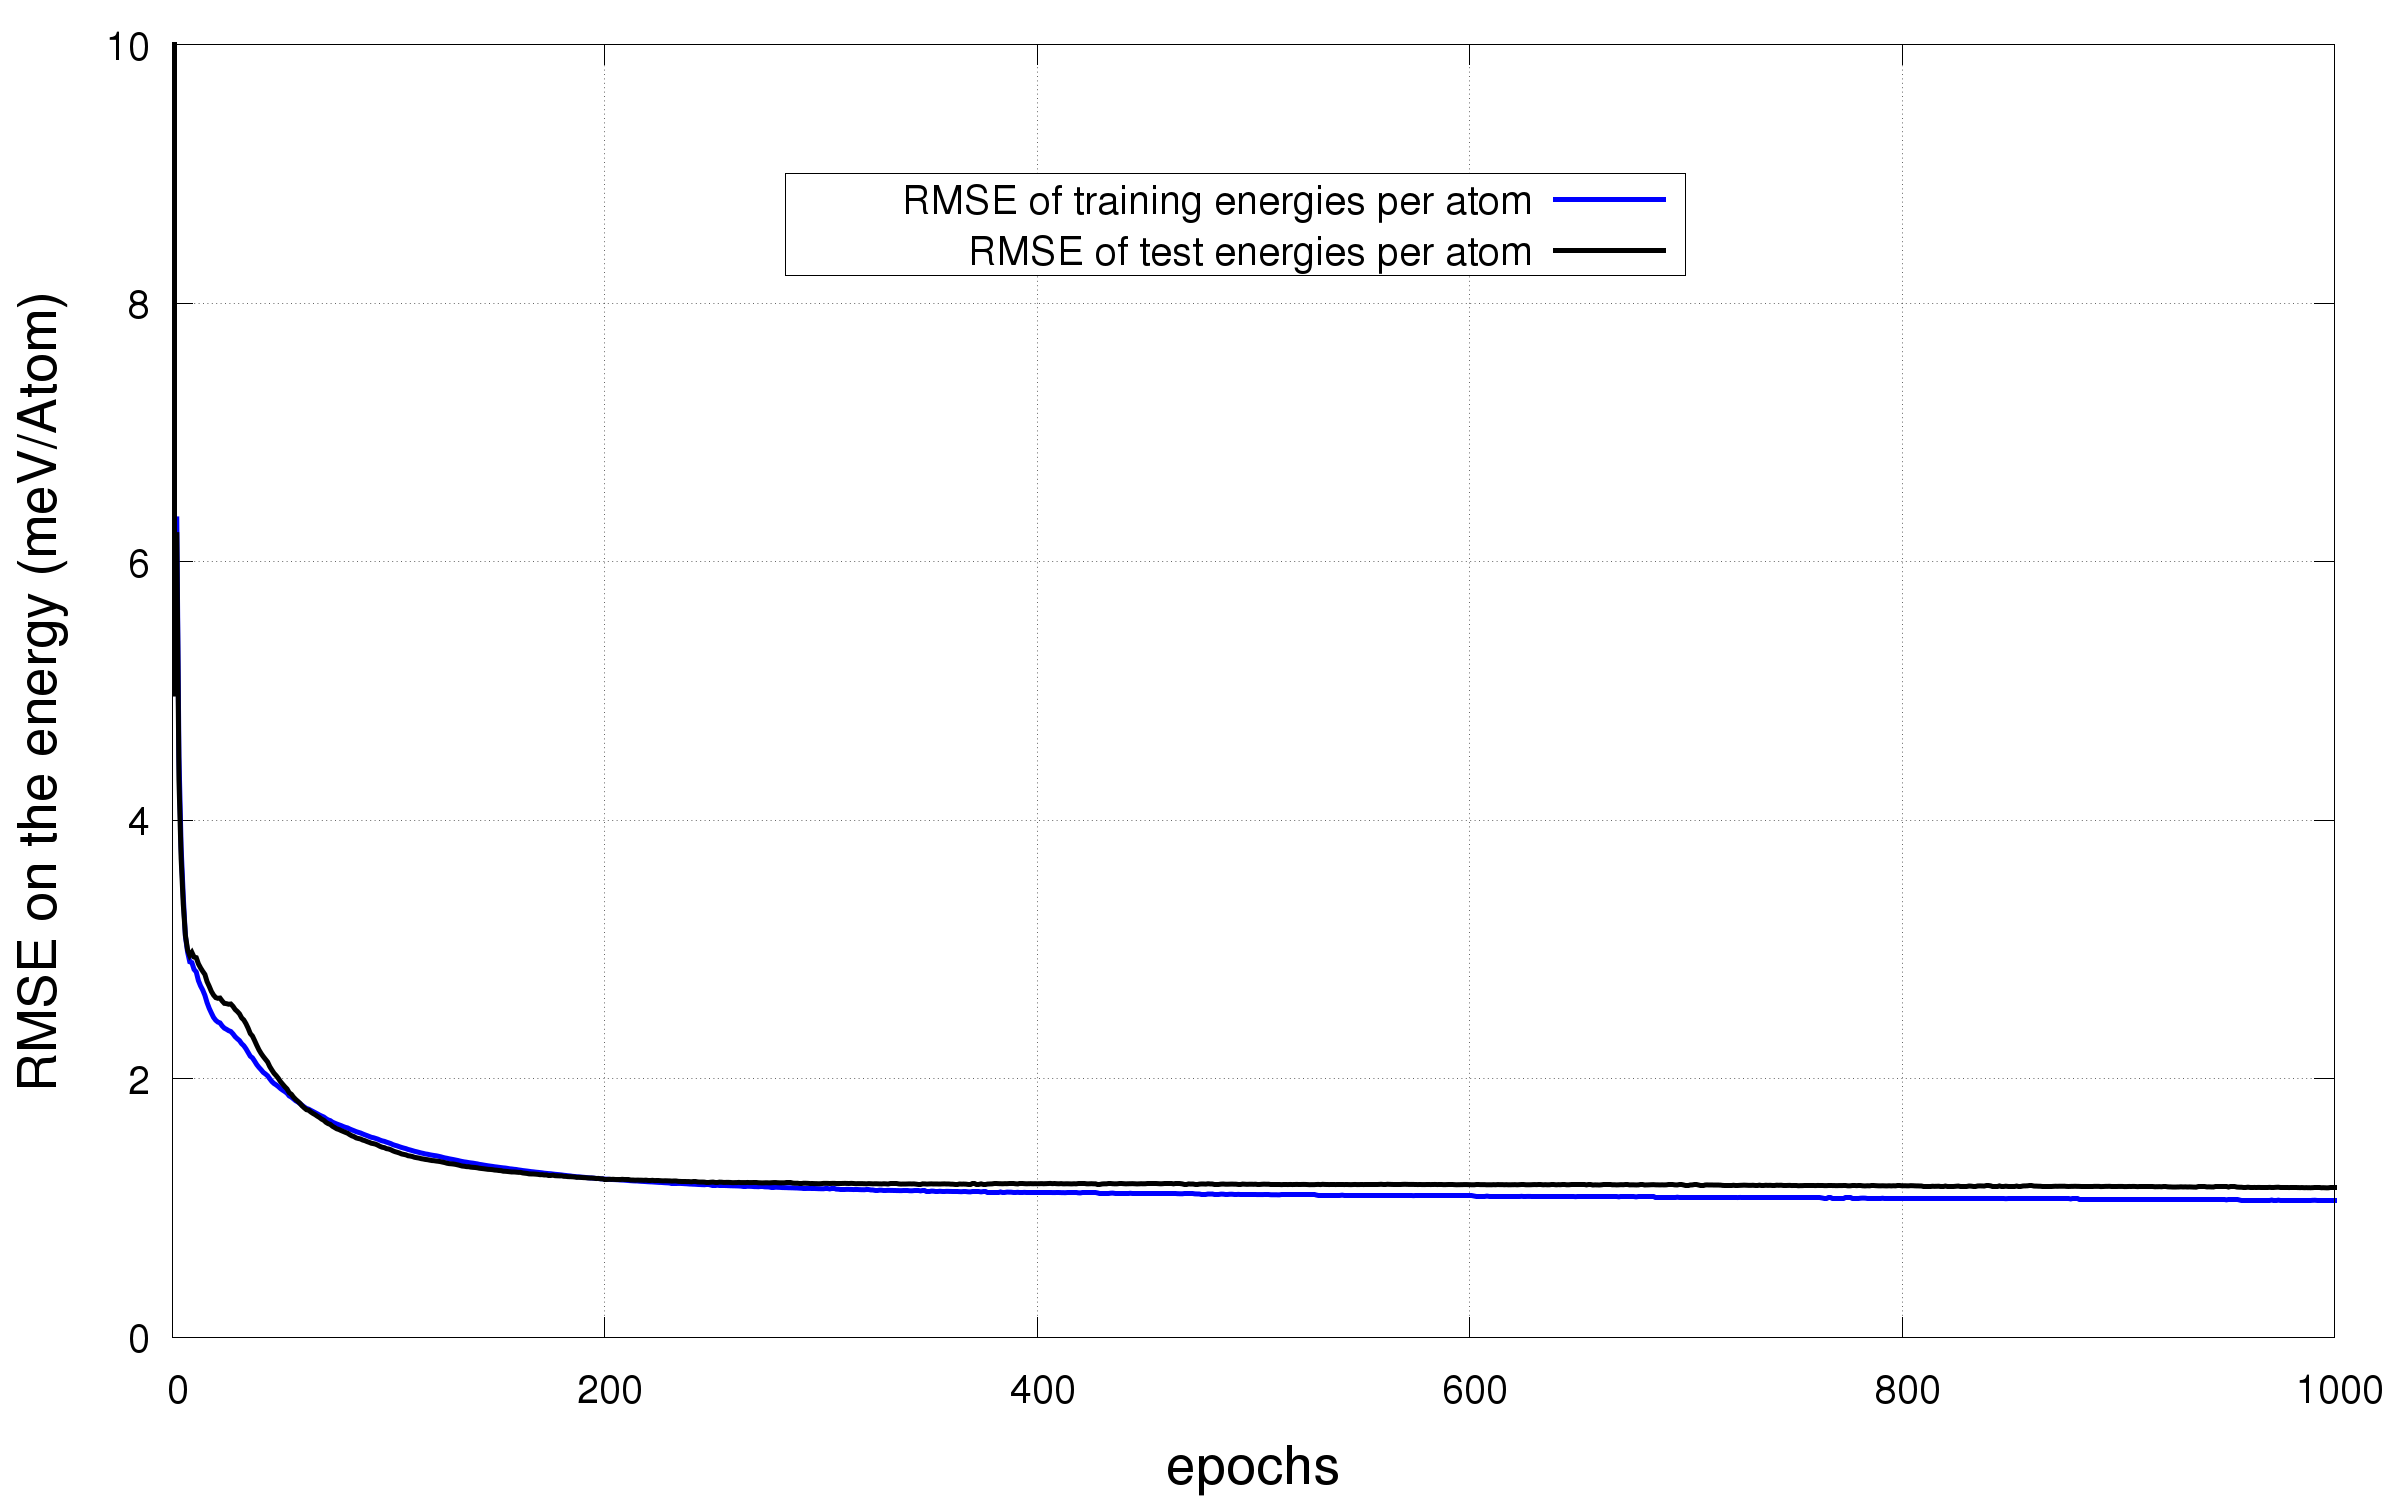
\includegraphics[scale=0.2]{energy.png}
    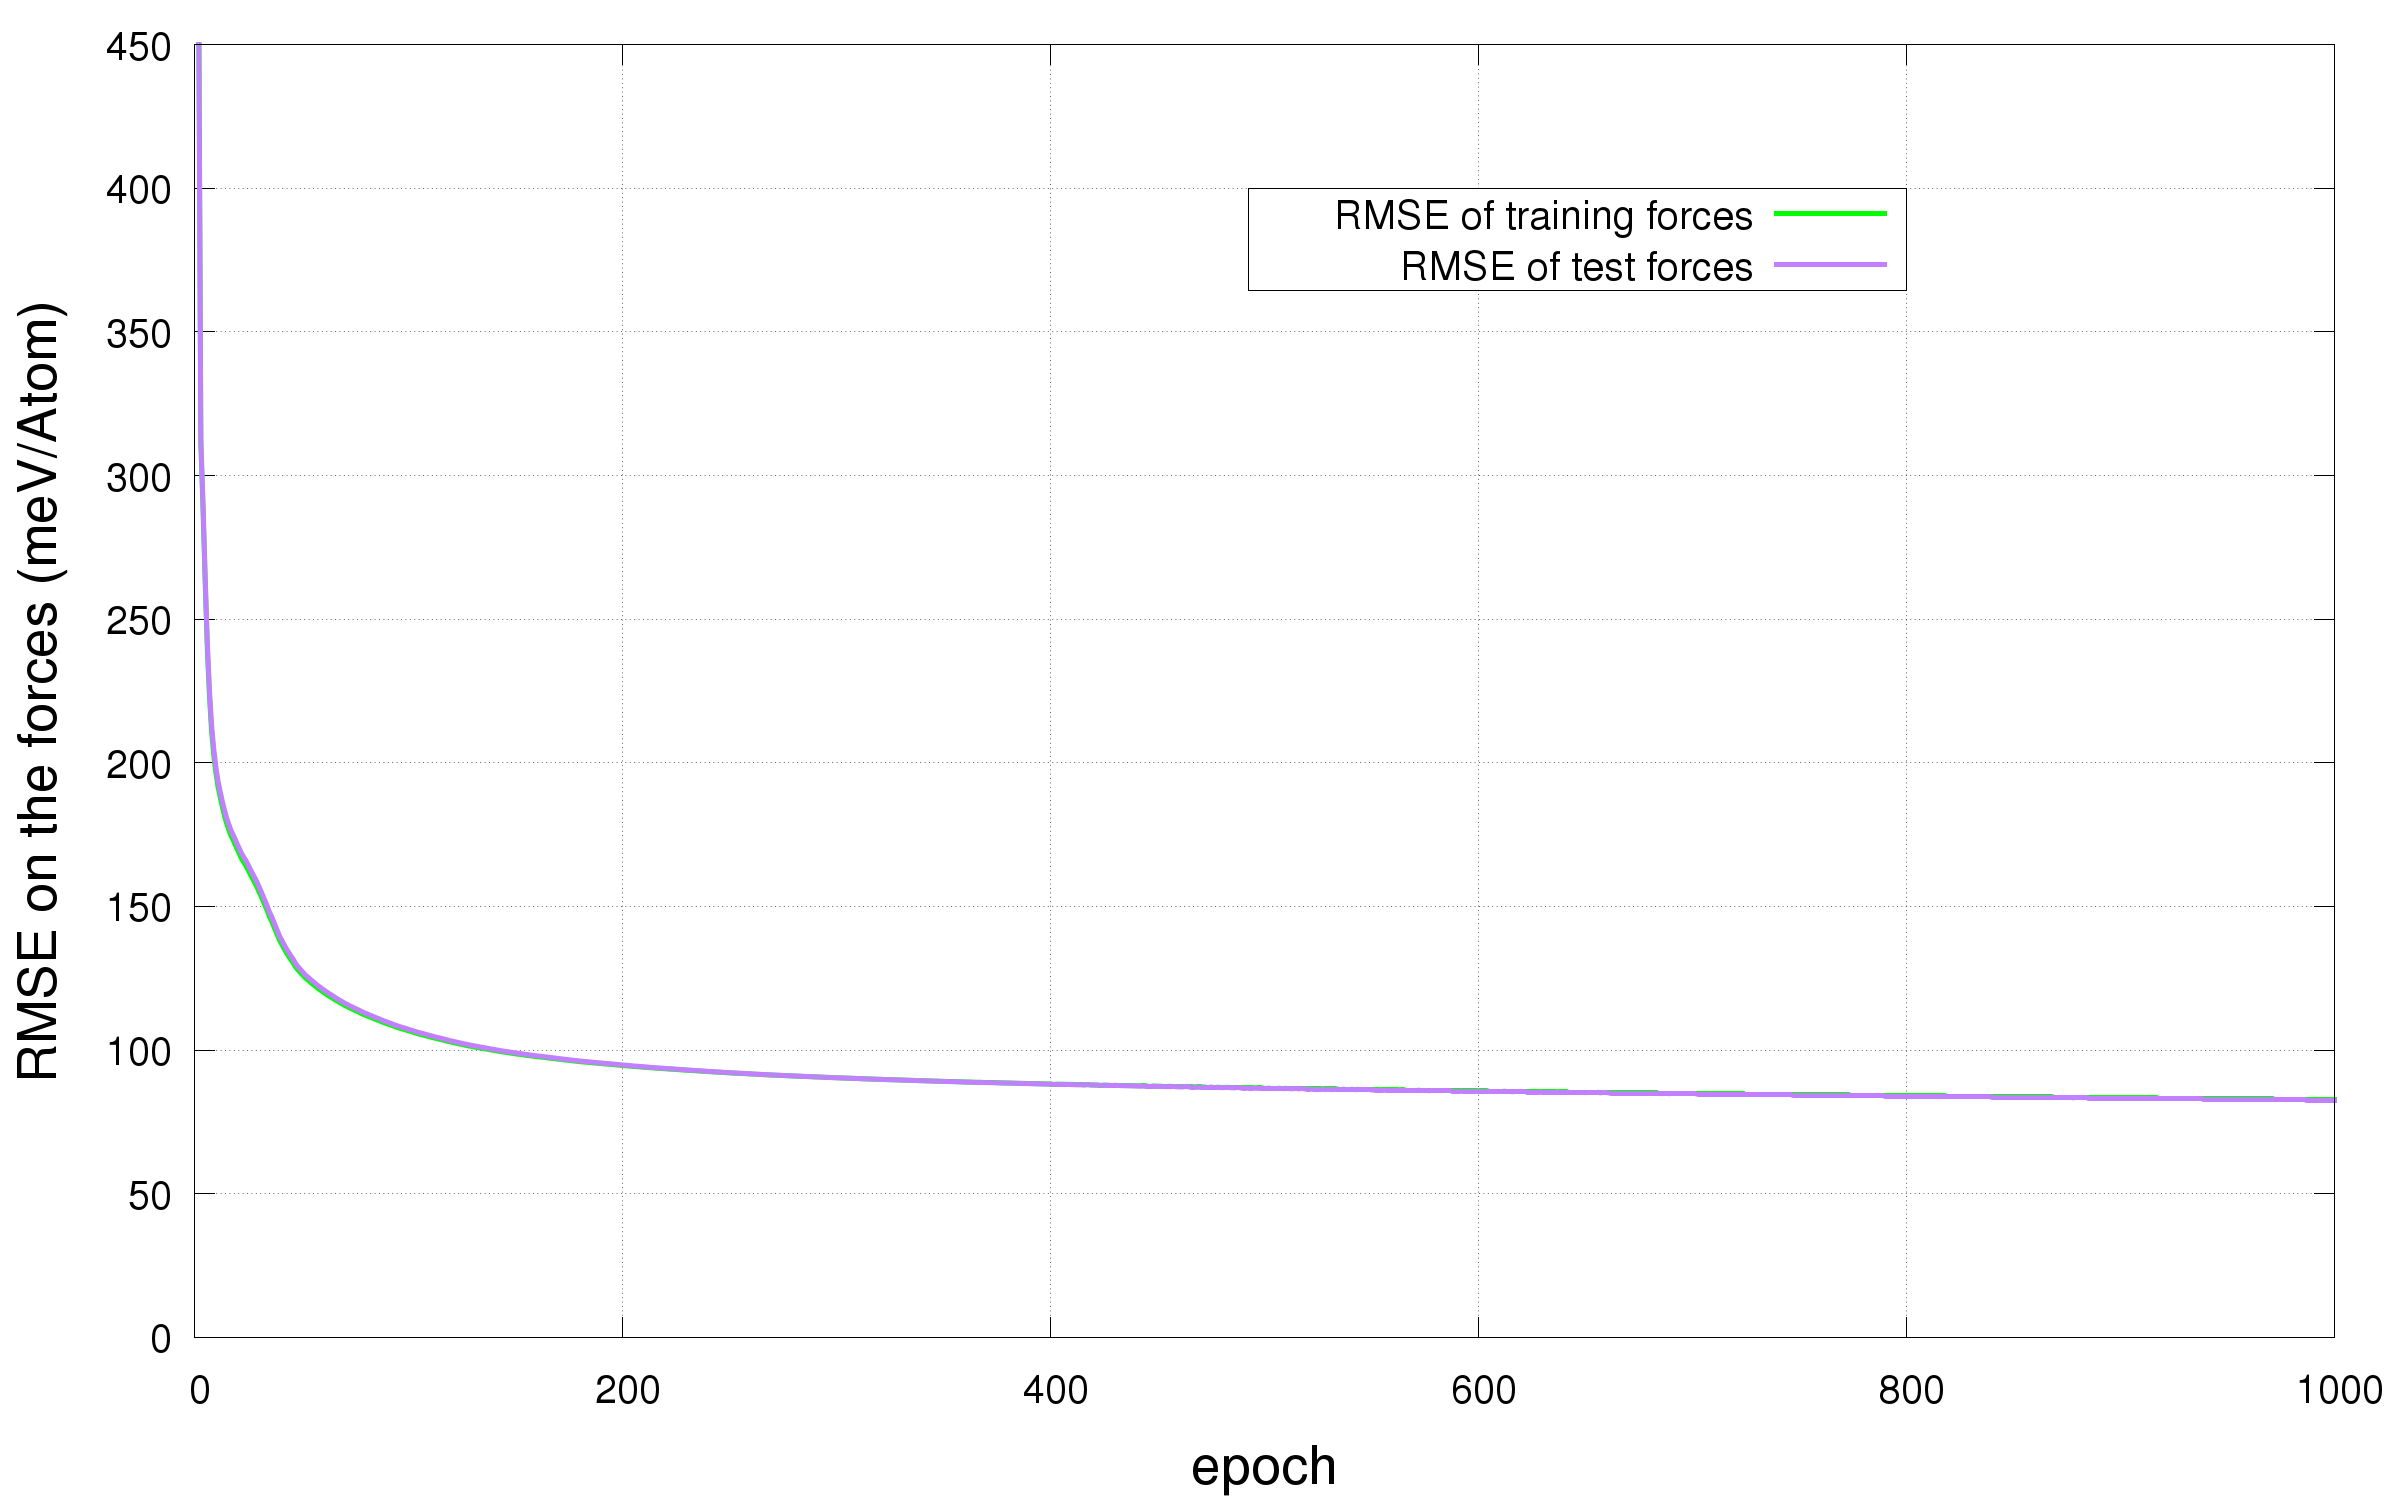
\includegraphics[scale=0.2]{forces.png}
    \caption{Energy (direct) and forces (direct) learning curves. The training has been performed on 800 structures and testing on 200 structures.}
    \label{fig:my_label}
\end{figure}
\\
\begin{mybox1}{Ratio between training and testing}
\Warning Be careful between the ratio taken into account in the training procedure, especially when you have a small database. The keyword in the input.nn responsible for such a parametrization is \textit{test\_fraction} and is set to 0.2 in our case. It means that 80\% of our total structures (2400 in this case) will be used for training while 20\% (600 in this case) will be used for testing. Normally, no strong differences should be observed between training and testing curves.  
\end{mybox1}

\begin{mybox1}{Interpretation tool !}
\begin{itemize}
    \item Errors for the energy and forces predictions are comprised around 1meV/Atom and 75meV/Atom. This is good when we compare it to our reference step (1 meV/Atom and 150 meV/Atom). 
    \item No differences are observed between testing and training curves for the energy and forces. 
\end{itemize}
\end{mybox1}

\begin{mybox3}{Output Files}
\begin{itemize}
    \item \textbf{learning-curve.out}
    \item \textbf{weights.001.001000.out}
    \item \textbf{weights.008.001000.out}
\end{itemize}
\end{mybox3}
%
\subsubsection{How to restart a Neural Network training ?}
%
Imagine either the simulation time was not enough to complete your calculation or you need to add more than the initial number of epoch, it should be desirable to be able to restart our calculation from the last iteration (here in this case epoch=1000). To perform this task, follow this procedure:
\begin{enumerate}
    \item create a new directory
    \item copy the input.data input.nn scaling.data weights.001.0001000.out weights.008.0001000.out files in this new directory
    \item move to this new directory
    \item add (or delete the \# symbole) the following keyword in the ADDITIONAL SETTINGS FOR TRAINING: \textit{use\_old\_weights\_short}
    \item launch your calculation similarly to the previous one using the \textcolor{green}{nnp--train} executable.
\end{enumerate}
%
%
%
\newpage
\fancyhead[L]{5. NNP--MD}
\section{Part 2: Link the direct NNP to Molecular Dynamics}
We finally generated our first NNP set. In order to improve it, we need to run it to detect non--physical structures. These ones will be then added to the NNP, which will be retrain and the procedure should be performed as a SCF procedure until no new structures are detected. \\
In our case, we would like to see how to link a "ready" NNP, this is why we will not use our NNP but another one already available in the n2p2 examples directory \textit{interface-LAMMPS/H2O\_RPBE-D3/nnp-data}.
%
\subsection{i--PI code}
Since we have a NNP able to reproduce accurately and fastly the forces and energies of water structures, it should be desirable to couple that to a Molecular Dynamics software. Two options are available to couple n2p2:
\begin{itemize}
    \item The LAMMPS software
    \item The CABANA software
\end{itemize}
Our choice in this tutorial is focused on the first, the LAMMPS software. Once this choice of coupling is done, we need now to efficiently couple both to optimize the simulation time. In this direction, the software i--PI is clearly designed to perform this task as it corresponds to a universal force engine for advanced molecular dynamics. i--PI is an interface for advanced molecular simulations written in Python, designed to be used together with an ab initio evaluation of the interactions between the atoms. The main goal is to decouple the problem of evolving the ionic positions to sample the appropriate thermodynamic ensemble and the problem of computing the inter-atomic forces. It could be thus linked to several software such as LAMMPS, which is our main interest in this tutorial. One other interest to use the i--PI interface is that it suitable for high sampling (Replica--exchange) and free energy computations (linkage with PLUMED available).
%
\subsection{Launching the i--PI interface}
\begin{mybox2}{{Input Files, Executables and Scripts}}
\begin{minipage}[c]{0.5\linewidth}
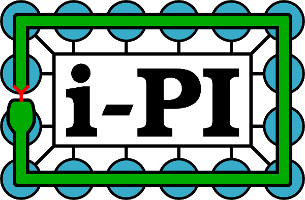
\includegraphics[scale=0.35]{ipi-logo-alpha.png}
\end{minipage}
\begin{minipage}[c]{0.5\linewidth}
\begin{itemize}
    \item input.xml
    \item system.xyz
\end{itemize}
\end{minipage}
\end{mybox2}
i--PI was designed for python 2 (even if a new version will be available as soon as possible for python 3), so please used for instance python2.7 to deal with it. Assuming the i--PI is in your directory, before any calculation you have to type in your directory the following command in order to launch the i--PI interface:
\begin{center}
\mybox{\textit{python2.7 i-pi input.xml $>>$ ipi.out \&}}
\end{center}
It will create an output file named ipi.out, and the i--PI interface will be waiting for any actions you will submit. This will be described in the next subsection. \\
Just a point on the input.xml file. It corresponds to the input file of i--PI and contain all the main informations of the MD, such as temperature, timestep, periodicity, units, thermodynamic ensemble, ...). You could feel free to change it if the conditions are not the same for another system of interest. The most critical block in this file is localized in the \textbf{prng} block with:
\begin{itemize}
    \item \textbf{socket}: keep driver--lammps1 if LAMMPS will be coupled to i--PI.
    \item \textbf{address}: it corresponds to the adress of the node where i--PI will be launched.
    \item \textbf{port}: the port of the node.
    \item \textbf{slots}: do not touch it.
    \item \textbf{timeout}: time for killing calculation without having any communications.
\end{itemize}

\begin{mybox3}{Output Files}
\begin{itemize}
    \item \textbf{ipi.out}
\end{itemize}
\end{mybox3}
%
\subsection{Linking n2p2 with LAMMPS}
\begin{mybox2}{{Input Files, Executables and Scripts}}
\begin{minipage}[c]{0.5\linewidth}
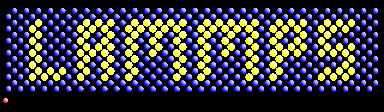
\includegraphics[scale=0.35]{LAMMPS.png}
\end{minipage}
\begin{minipage}[c]{0.5\linewidth}
\begin{itemize}
    \item lmp1.in
    \item system.xyz
    \item \textcolor{red}{get\_lammps.sh}
\end{itemize}
\end{minipage}
\end{mybox2}
Once i--PI is running and is waiting for communication with another software(s), we can initialize LAMMPS computation which will serve as an intermediate with n2p2 to compute energy and forces at every timestep of the dynamics and communicate them to i--PI for forces integration. We thus start with classical LAMMPS files, which have to be:
\begin{itemize}
    \item An input file (.in) where keyword for MD is specified,
    \item A coordinate file (.data), which is specific for LAMMPS.
\end{itemize}
Starting from a classical xyz structure, we could translate it in .data file by applying the \textcolor{red}{get\_lammps.sh} script as:
\begin{center}
\mybox{\textit{sh get\_lammps.sh system.xyz}}
\end{center}
Just adapt (if necessary) the script file in function of your system ! In our case, it is designed for our periodic box of water molecules, and an output file named \textbf{initial.data} is generated and correspond to the initial set of coordinates for the LAMMPS calculation. This file is called in lmp1.in as \textit{read\_data ./initial.data}, and mass objects are ordered in function of the initial.data file. For the other lines, a classical example is provided in the lmp1.in and is close to every input file for MD (AMBER, NAMD, Tinker, ...). For more details, a tutorial of LAMMPS will be specified at the end of the tutorial. \\
While i--PI is running and the initial.data and lmp1.in are ready for a LAMMPS calculation, additional keywords have to be added in the lmp1.in to specify the connection between LAMMPS and n2p2:
\begin{itemize}
    \item variable runnerCutoff    equal  7.0000
    \item variable runnerDir       string "/path/to/nnp-data"
    \item pair\_style nnp dir \$\{runnerDir\} showew no showewsum 1 resetew yes maxew 200000 cflength 1.889726 cfenergy 0.036749
    \item pair\_coeff * * \$\{runnerCutoff\}
    \item fix 1 all ipi 192.168.100.1 8766
\end{itemize}
The two first lines are variable declarations. \$\{runnerDir\} is the directory of the nnp data and \$\{runnerCutoff\} is maximum cutoff radius of all symmetry functions. \textbf{The cutoff must be given in LAMMPS length units, even if the neural network potential has been trained using a different unit system}. \\
The pair\_style adds an interaction based on the high-dimensional neural network potential method. It uses an interface to the NNP library, which has to be declared before launching the calculation (see next subsection). \\
Finally, the fix line called the adress and the port where i--PI is running.
\\
\begin{mybox3}{Output Files}
\begin{itemize}
    \item \textbf{initial.data}
\end{itemize}
\end{mybox3}
%
\subsection{Launching LAMMPS with the i--PI interface}
\begin{mybox2}{{Input Files, Executables and Scripts}}
\begin{minipage}[c]{0.5\linewidth}
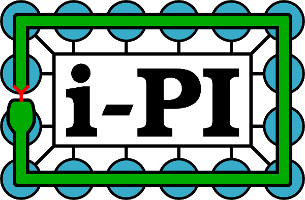
\includegraphics[scale=0.35]{ipi-logo-alpha.png}
\end{minipage}
\begin{minipage}[c]{0.5\linewidth}
\begin{itemize}
    \item lmp1.in
    \item initial.data
    \item \textcolor{blue}{nnp--data} directory
    \item \textcolor{green}{lmp}
\end{itemize}
\end{minipage}
\end{mybox2}
Create the nnp--data directory and place in the following files: input.data, input.nn, scaling.data, weights.XXX.001000.out and change the respective weights001.001000.out and weights008.001000.out by weights.001.data and weights.008.data. \\
Once the lmp1.in and the nnp data directory are ready, just follow these instructions to launch your calculation:
\begin{enumerate}
    \item export LD\_LIBRARY\_PATH=/path/to/n2p2/lib:\$\{LD\_LIBRARY\_PATH\}
    \item lmp -i lmp1.in $>>$ log1.lammps \&
\end{enumerate}
Files \textbf{simulation.force\_0.xyz} and \textbf{simulation.pos\_0.xyz} will be filled, according to the printing frequency we specified in the lmp1.in (here 1 at the "fix" line).
\\
\begin{mybox1}{Interpretation tool !}
\begin{itemize}
    \item Simulation could be observed using either vmd or molden softwares. It is the first step to do in order to observe if the simulation is stable or not.
    \item From this simulation, new structures could then be extracted to improve the quality of the NNP, and training as well as simulations are then performed in a SCF procedure until no new structures are observed.
\end{itemize}
\end{mybox1}
%
\fancyhead[L]{6. Baselined NNP--MD}
\section{Part 3: From direct to baselined NNP}
%
\subsection{What is baselined NNP?}
In the previous sections (parts 1 and 2) we learnt how to generate a NNP and how to use it within the i--PI interface. While the NNP trained directly on DFT data provide predictions at impressive speed, the stability and accuracy of these NNPs is often difficult to achieve. The problems with stability are probably the simplest ones to detect. The system simulated with non-stable NNPs has tendency to explode within the first picosecond of the simulation. The reasons might be:
\begin{enumerate}
    \item \textbf{The quality of the generated data}: instead of generating initial structures with the Tinker MD software, we could use semi--empirical methods to generate structures more closely to \textit{ab initio} dynamics. 
    \item \textbf{The choice of symmetry functions}: the number as well as the spacing chosen to generate the symmetry functions play a crucial role in the stability of the NNP. 
    \item \textbf{Number of data points}: Direct NNP require relatively large number of structures to provide stable dynamics. Low nuber of the structures can be reason for instabilities in sparsely represented regions of PES.
\end{enumerate}
As demonstarted by the examples, stabilization of direct NNPs is not an easy task, even for a small water box. A suitable alternative is to train so called baselined NNP. Instead of reproducing directly the DFT forces and energy, the NNPs are trained to correct the forces and energy computed at a lower level of theory, for example semiempirical method. The baselined NNPs require lower number of structures and descriptors and more robust compared to the direct NNP. In the following part, we show how to adapt our NNP training protocol in order to use it as a "Baselined NNP". 
%
\subsection{Baselined forces and energy}
\begin{mybox2}{{Input Files, Executables and Scripts}}
\begin{minipage}[c]{0.5\linewidth}

\includegraphics[scale=0.15]{xtb.png}
\end{minipage}
\begin{minipage}[c]{0.5\linewidth}
\begin{itemize}
    \item input.data
    \item \textcolor{green}{xtb}
\end{itemize}
\end{minipage}
\end{mybox2}
While we already have the accurate reference energies and forces coming from the cp2k computations, we need to choose suitable baseline method. In this tutorial, we use semiempirical GFN0-xTB method. Therefore, energy and forces of the training structures need to be recomputed at this level. \\
To proceed to the computations, please follow these steps:
\begin{enumerate}
    \item Create one folder per structure and extract the corresponded structure from the input.data file and place it in the corresponded folder (\textit{prep.sh})
    \item Convert each frame (n2p2 format) in xyz format (\textit{prep2.sh} linked with \textit{from\_data\_to\_xtb.f90})
    \item Submit interactively all the computations at the GFN0-xTB level of theory (\textit{sub.sh})
    \item Once all the computations are ended, compute the differences between DFT and GFN0-xTB energies and forces for each frame and add the results in a new file called new--input.data (\textit{calc--diff.sh}).
\end{enumerate}

\begin{mybox3}{Output Files}
\begin{itemize}
    \item \textbf{new--input.data}
\end{itemize}
\end{mybox3}
%
\subsection{New training}
\begin{mybox2}{{Input Files, Executables and Scripts}}
\begin{minipage}[c]{0.5\linewidth}

\includegraphics[scale=0.1]{n2p2.png}
\end{minipage}
\begin{minipage}[c]{0.5\linewidth}
\begin{itemize}
    \item new--input.data
    \item input.nn
    \item \textcolor{green}{nnp--scaling}
    \item \textcolor{green}{nnp--train}
\end{itemize}
\end{minipage}
\end{mybox2}
First, rename the new--input.data to input.data and place it in a new folder with the input.nn file. The procedure to train a Baselined--NNP is analogous to direct NNP:
\begin{enumerate}
    \item Use the \textcolor{green}{nnp--scaling} executable (see Step 4) to generate the corresponding scaling.data
    \item Use the \textcolor{green}{nnp--train} executable (see Step 4 again) to train Baselined--NNP. 
\end{enumerate}

\begin{mybox3}{Output Files}
\begin{itemize}
    \item \textbf{learning-curve.out}
    \item \textbf{weights.001.001000.out}
    \item \textbf{weights.008.001000.out}
\end{itemize}
\end{mybox3}
%
\subsection{Baselined--NNP with i--PI}
\begin{mybox2}{{Input Files, Executables and Scripts}}
\begin{minipage}[c]{0.5\linewidth}
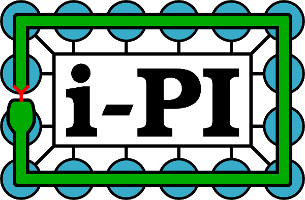
\includegraphics[scale=0.35]{ipi-logo-alpha.png}
\end{minipage}
\begin{minipage}[c]{0.5\linewidth}
\begin{itemize}
    \item input.data // input.nn // scaling.data
    \item weights.001.001000.out // weights.008.001000.out
    \item input.xml
    \item initial.data // system.xyz
    \item lmp1.in
    \item \textcolor{green}{xtb\_ase.py} // xtb\_io.py
\end{itemize}
\end{minipage}
\end{mybox2}

Once the training is finished, you can launch your Baselined--NN MD similarly to direct NNP. The main difference is that apart from the NNP itself, you also need to perform computation of the baseline ate every step. The submission is  be done as follows: 
\begin{enumerate}
    \item Create a new directory labeled nnp--data and place there the input.data, input.nn, scaling.data and weightsXXX.data files from the last epoch
    \item Change the name of the weightsXXX.data files in respectively weights.001.data (H) and weights.008.data (O).
    \item Adapt the path of the nnp--data folder in the lmp1.in file
    \item Also adapt the sockets in the respectively files:
    \begin{itemize}
        \item input.xml
        \item lmp1.in
        \item xtb\_ase.py
        \item sub.run
    \end{itemize}
    \item Launch the simulation with the sub.sh script file !
\end{enumerate}

\begin{mybox1}{New xtb--ase python interface}
\begin{itemize}
    \item The both files \textcolor{green}{xtb\_ase.py} and xtb\_io.py provide a new python interface between ase and xtb as the interface for xtb 6.3.3 encounters some issues ...
    \item This interface is a little bit primitive, so be careful about error messages ...
\end{itemize}
\end{mybox1}

\begin{mybox1}{Interpretation tools}
\begin{itemize}
    \item This time, the simulation does not crash as it was the case for the direct NNP. It finally means that direct NNP is definitevely more sensitive to the choice of symmetry functions as well as initial structures encompassing the dataset. 
    \item However, the EW messages present in the log.lammps are too high ... (around 50 EW per step in our cas). \textbf{A rule of thumb is to consider that a structure depicted more than 10/20 EW is badly described by the NNP}. It means that even if the simulation does not crash, the NNP is not optimal and should be optimized following the self consistent procedure described in section 2 of this tutorial.
\end{itemize}
\end{mybox1}
%
\subsection{Fast and accurate: Multiple-time-step approach}
\begin{mybox2}{{Input Files, Executables and Scripts}}
\begin{minipage}[c]{0.5\linewidth}
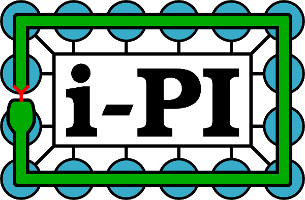
\includegraphics[scale=0.35]{ipi-logo-alpha.png} \\
\end{minipage}
\begin{minipage}[c]{0.5\linewidth}
\begin{itemize}
    \item input.data // input.nn // scaling.data from baselined
    \item input.data // input.nn // scaling.data from direct
    \item weights.001.001000.out // weights.008.001000.out from baselined
    \item weights.001.001000.out // weights.008.001000.out from direct
    \item input.xml
    \item initial.data // system.xyz
    \item lmp1.in
    \item \textcolor{green}{xtb\_ase.py} // xtb\_io.py
\end{itemize}
\end{minipage}
\end{mybox2}
When direct NNP is not stable to fully run itself but not so bad in single point accuracy, it could be coupled to the baselined NNP to form what we call a mulit--time--step approach. In this approach, forces and energy are computed x times using the direct NNP and then one time with the baselined NNP. It helps to avoid some crashing from the direct NNP and improves the speed of the simulation because the baselined is not computed at every step. Using the i--PI software, we will see how such a coupling is possible. 


To run i--PI within such a mode (i.e multi--time--step), please follow the following instructions:
\begin{enumerate}
    \item Create a folder and place the submission file, system.xyz and input.xml files
    \item In this folder, create two new directories labeled nnp-data-direct and nnp-data-baselined and place in each respective folder the corresponding input.data, input.nn, scaling.data and the weights.XXX.data files
    \item Place the lmp1.in in both the directories and adapt the respective path of the corresponding folder in each lmp1.in
    \item Do not forget to place xtb\_ase.py and xtb\_io.py in the baselined directory
    \item Adapt the sockets in input.xml and lmp1.in for the direct NNP
    \item Adapt the sockets in input.xml, lmp1.in and xtb\_ase.py for the baselined NNP
    \item Launch the simulation with the sub.sh script file !
\end{enumerate}
In our case, we launched a multi--time--step simulation with an inner timestep of 0.5 fs where forces and energy are computed with the direct NNP and an outer timestep of 3 fs where forces and energy are computed using the xTB baseline and corrected with the baselined NNP. All the relative keywords are mentioned within the input.xml and the structure of the file does not differ from the previous ones met during the tutorial.
\begin{mybox1}{Interpretation tools}
\begin{itemize}
    \item The accuracy of such a dynamic is very sensitive to the energy conservation during the dynamics. Therefore, the choice of 0.5/3 was made in a sens to ensure the conservation of the energy. However on other systems careful attention should be taken on this conservation.
    \item As mentioned before EW should still be checked but should be now lower compared to the direct NNP simulation. 
    \item Finally, in order to improve the accuracy from the baselined more than 1 NNP can be considered during the dynamics. Indeed, i--PI enables to take the average made on more than 1 prediction. It has the main advantage to decrease the error made on the NNP prediction but impact the speed of the dynamics as more predictions has to be performed at the same time.
\end{itemize}
\end{mybox1}
%
%
\newpage
\fancyhead[L]{7. Conclusions and supplementary tutorials}
\section{Conclusions}
Thorough this tutorial we described the main idea on how to construct manually an efficient NNP and how to link it to a MD software (LAMMPS in our case). This procedure is straightforwardly transferable to every chemical systems and hope it will be helpful to include reactivity in conventional Molecular Dynamics.  
%
\section{Supplementary tutorials}
\label{sec:tutorials}
A list of supplementary tutorials is given to help users if questions appear (espcially in the input files of several softwares).
\subsection{Tinker(--HP)}
\begin{itemize}
    \item Frédéric CELERSE personnal tutorials (on request): cMD / preparing Tinker xyz files / Umbrella Sampling / Steered Molecular Dynamics / Gaussian accelerated Molecular Dynamics
    \item AMOEBA workshop: \url{https://sites.google.com/site/amoebaworkshop/}
    \item Tinker website: \url{https://dasher.wustl.edu/tinker/}
    \item GitHub (open source code): \url{https://github.com/TinkerTools/tinker}
\end{itemize}
\subsection{n2p2}
\begin{itemize}
    \item GitHub (open source code): \url{https://github.com/CompPhysVienna/n2p2}
    \item Short tutorial: \url{https://compphysvienna.github.io/n2p2/index.html}
\end{itemize}
\subsection{cp2k}
\begin{itemize}
    \item GitHub (open source code): \url{https://github.com/cp2k/cp2k}
    \item cp2k main website: \url{https://www.cp2k.org/}
\end{itemize}
\subsection{i--PI}
\begin{itemize}
    \item GitHub (open source code): \url{https://github.com/i-pi/i-pi}
    \item i--PI website: \url{http://ipi-code.org/}
    \item i--PI manual: \url{http://ipi-code.org/assets/pdf/manual.pdf}
\end{itemize}
\subsection{LAMMPS}
\begin{itemize}
    \item GitHub (open source code): \url{https://github.com/lammps/lammps}
    \item LAMMPS website: \url{https://lammps.sandia.gov/}
    \item LAMMPS tutorials: \url{https://icme.hpc.msstate.edu/mediawiki/index.php/LAMMPS_tutorials.html}
\end{itemize}

\newpage
\fancyhead[L]{9. Optimal protocol for stable NNP}
\section{Optimal protocol for stable NNP}
In this last section, we aim at providing optimal parameters to train a NNP which could be then used for production. Note that the proposed methods and parameters come from different works available in the literature and modifications might be needed. 

\textbf{SYSTEM CASE}: The user want to model a direct NNP of an azobenzene in order to reproduce an \textit{ab--initio} MD. In this case, the user has to separate two important components:
\begin{enumerate}
    \item How he will built his own NNP ?
    \item How he will train for ?
\end{enumerate}
These two features are complementary but have to be treated carefully and separated. Let us see how we suggest to proceed for that !
\subsection{How to build a good starting NNP ?}
The complexity as well as the chemical event that any user would like to explore are two crucial parameters to take into account. Here, there is only 3 different atom types (H,C and N) and the system is made of 24 atoms. In case of the photoswitches, the event could be decoupled into two main parts:
\begin{enumerate}
    \item \textbf{PHOTO}: a photo event comes from by an photo-excitation of the system through any wave length. 
    \item \textbf{SWITCH}: a switch event is related to the conformation switch of a molecule which is only due to thermal fluctuations.
\end{enumerate}
In our case, the photo part needs some external excitations, which is not available in MD--NN based only on the ground state Potential Energy Surface. Concerning the switch part, we have two available conformations: E and Z. One interesting question should be thus: \textbf{Which mechanic way should enable the switch of azobenzene from E to Z ?} \\
To answer to this question, we need thus to prepare the NN according to this specific question. In our case, and according to the literature, azobenzene could depict two switch mechanisms: the inversion and the rotation. The aim is thus to let the choice of the desired path within our MD--NN to observe which way is preferred or not. Therefore, the NN has to know the existence of these two ways and structures taken to build the NN should be part of these pathways. \\
To generate these structures, you can follow the following instructions:
\begin{enumerate}
    \item For each pathway, generate a metadynamics of several ns using a baselined (DFTB+, xTB) using i--Pi coupled to the baselined and plumed,
    \item Extract the most relevant structures either manually or by using a clustering method (PCA, TICA, TSNE, ...)
    \item Only for the most important structures, run a Replica Exchange MD of several ps in order to capture the fluctuation effects from the temperature. Extract as before the most relevant structures.
\end{enumerate}
Once all the structures extracted, we can grab them in order to generate the first dataset which will be used as a starting point for the procedure. Note that a good compromise for the number of structures to start is localized between 5000 (for simple system) and 10 000 (for more complex system). 
%
\subsection{How to efficiently train a good NNP ?}
Once the initial dataset was created, the other important part of the work is to design the architecture for future NNP.
\end{document}